% Options for packages loaded elsewhere
\PassOptionsToPackage{unicode}{hyperref}
\PassOptionsToPackage{hyphens}{url}
%
\documentclass[
  12pt,
  a4paper,
]{ctexart}
\usepackage{amsmath,amssymb}
\usepackage{lmodern}
\usepackage{iftex}
\ifPDFTeX
  \usepackage[T1]{fontenc}
  \usepackage[utf8]{inputenc}
  \usepackage{textcomp} % provide euro and other symbols
\else % if luatex or xetex
  \usepackage{unicode-math}
  \defaultfontfeatures{Scale=MatchLowercase}
  \defaultfontfeatures[\rmfamily]{Ligatures=TeX,Scale=1}
\fi
% Use upquote if available, for straight quotes in verbatim environments
\IfFileExists{upquote.sty}{\usepackage{upquote}}{}
\IfFileExists{microtype.sty}{% use microtype if available
  \usepackage[]{microtype}
  \UseMicrotypeSet[protrusion]{basicmath} % disable protrusion for tt fonts
}{}
\makeatletter
\@ifundefined{KOMAClassName}{% if non-KOMA class
  \IfFileExists{parskip.sty}{%
    \usepackage{parskip}
  }{% else
    \setlength{\parindent}{0pt}
    \setlength{\parskip}{6pt plus 2pt minus 1pt}}
}{% if KOMA class
  \KOMAoptions{parskip=half}}
\makeatother
\usepackage{xcolor}
\IfFileExists{xurl.sty}{\usepackage{xurl}}{} % add URL line breaks if available
\IfFileExists{bookmark.sty}{\usepackage{bookmark}}{\usepackage{hyperref}}
\hypersetup{
  pdftitle={问题三：可解释性多模态情感预测},
  hidelinks,
  pdfcreator={LaTeX via pandoc}}
\urlstyle{same} % disable monospaced font for URLs
\usepackage[margin=2.5cm]{geometry}
\usepackage{longtable,booktabs,array}
\usepackage{calc} % for calculating minipage widths
\usepackage{needspace}
\raggedbottom
\sloppy
% Correct order of tables after \paragraph or \subparagraph
\usepackage{etoolbox}
\makeatletter
\patchcmd\longtable{\par}{\if@noskipsec\mbox{}\fi\par}{}{}
\makeatother
% Allow footnotes in longtable head/foot
\IfFileExists{footnotehyper.sty}{\usepackage{footnotehyper}}{\usepackage{footnote}}
\makesavenoteenv{longtable}
\usepackage{graphicx}
\makeatletter
\def\maxwidth{\ifdim\Gin@nat@width>\linewidth\linewidth\else\Gin@nat@width\fi}
\def\maxheight{\ifdim\Gin@nat@height>\textheight\textheight\else\Gin@nat@height\fi}
\makeatother
% Scale images if necessary, so that they will not overflow the page
% margins by default, and it is still possible to overwrite the defaults
% using explicit options in \includegraphics[width, height, ...]{}
\setkeys{Gin}{width=\maxwidth,height=\maxheight,keepaspectratio}
\setkeys{Gin}{width=.92\linewidth,height=.70\textheight,keepaspectratio}
% Set default figure placement to htbp
\makeatletter
\def\fps@figure{p}
\makeatother
\setlength{\emergencystretch}{3em} % prevent overfull lines
\providecommand{\tightlist}{%
  \setlength{\itemsep}{0pt}\setlength{\parskip}{0pt}}
\setcounter{secnumdepth}{-\maxdimen} % remove section numbering
\ifLuaTeX
  \usepackage{selnolig}  % disable illegal ligatures
\fi

\title{问题三：可解释性多模态情感预测}
\author{}
\date{}

\begin{document}
\hypertarget{ux95eeux9898ux4e09ux53efux89e3ux91caux6027ux591aux6a21ux6001ux60c5ux611fux9884ux6d4b}{%
\section{问题三：可解释性多模态情感预测}\label{ux95eeux9898ux4e09ux53efux89e3ux91caux6027ux591aux6a21ux6001ux60c5ux611fux9884ux6d4b}}

\hypertarget{ux95eeux9898ux5206ux6790ux4e0eux5efaux6a21ux76eeux6807}{%
\subsection{1
问题分析与建模目标}\label{ux95eeux9898ux5206ux6790ux4e0eux5efaux6a21ux76eeux6807}}

问题三要求在三模态信息完整的条件下，同时输出情感极性、情感强度以及能够回溯到原始素材的解释证据。模型不仅要回答``样本属于哪一类、强度是多少''，还要回答``文本、语音和视觉分别起到了多大作用，以及哪一段信息改变了当前判断''。因此，本问题被建模为一个带有后验反事实解释的多任务学习问题。

三模态具有不同的特征维度、时间组织方式和有效长度。直接拼接可能造成高维文本特征主导训练，也可能使填充位置参与注意力计算。另一方面，模型内部的注意力和门控值只反映表征交互或融合状态，不能单独证明某个片段真正影响了最终输出。本文据此采用如下路线：先在训练集边界内完成标准化，再进行掩码感知的模态内时序编码；以文本为查询完成音频和视觉交互；通过动态门控获得样本级融合表示；利用分类头和回归头联合预测；最后固定模型参数，以训练集均值为反事实基线，执行模态级和局部窗口级遮挡，生成贡献度、证据映射、关键帧和解释卡。

\begin{figure}
\hypertarget{fig:route}{%
\centering
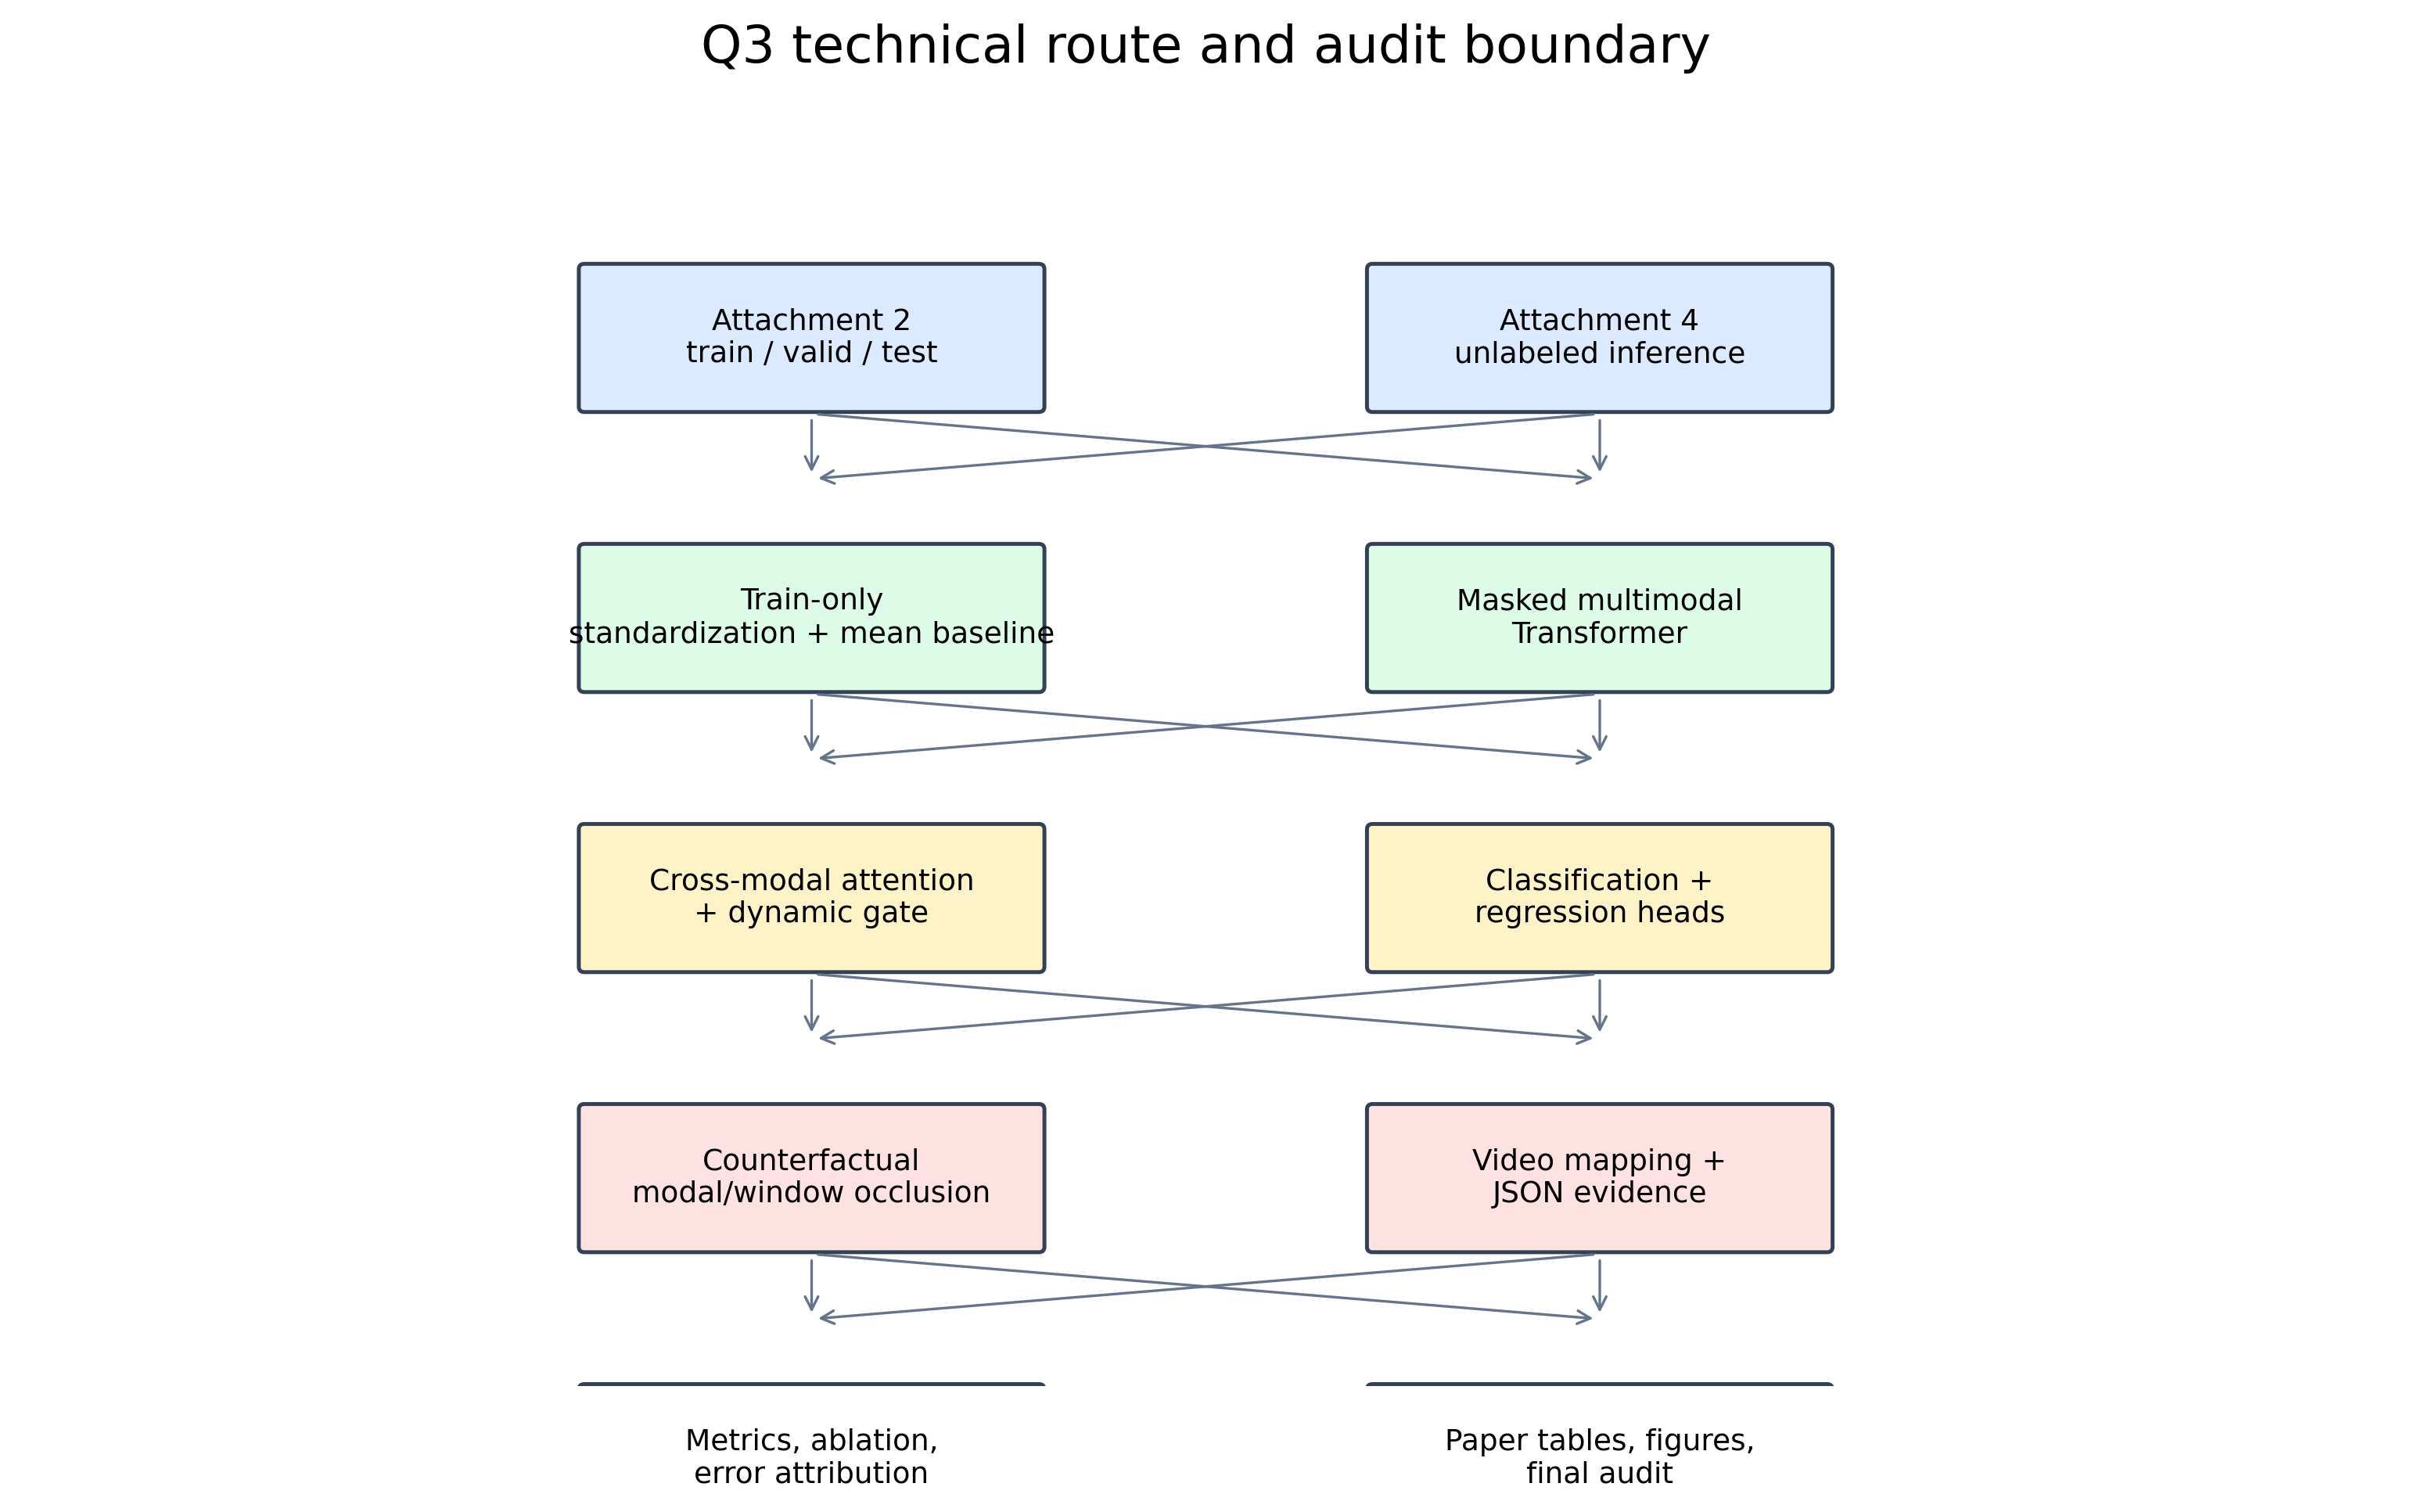
\includegraphics{assets/fig_technical_route.png}
\caption{问题三技术路线}\label{fig:route}
}
\end{figure}

图 1
展示了从特征输入到证据输出的完整流程。图中预测主干和解释分支共享同一个最佳模型，解释阶段不再更新模型参数，也不使用附件四选择超参数。

\hypertarget{ux6a21ux578bux5047ux8bbeux4e0eux7b26ux53f7ux5b9aux4e49}{%
\subsection{2
模型假设与符号定义}\label{ux6a21ux578bux5047ux8bbeux4e0eux7b26ux53f7ux5b9aux4e49}}

\hypertarget{ux6a21ux578bux5047ux8bbe}{%
\subsubsection{2.1 模型假设}\label{ux6a21ux578bux5047ux8bbe}}

（1）每个样本的文本、语音和视觉信息均可表示为保序时序序列，序列位置的相对关系包含情感表达信息。

（2）特征文件提供的有效掩码能够区分有效观测、填充位置和无效位置；掩码同时作用于自注意力、跨模态注意力和池化。

（3）预处理统计量只由训练集估计，验证集、测试集和附件四复用训练集统计量。

（4）情感极性和强度共享多模态语义表示，但使用独立输出头，因为分类边界和连续强度并不等价。

（5）遮挡模态或局部窗口后产生的预测变化表示模型敏感性，不等同于真实情感成因或人类心理因果关系。

（6）对齐特征的相同序号表示相对对齐窗口，不保证逐词、逐帧的真实时间戳；文本证据因而只报告对齐相对窗口。

\hypertarget{ux7b26ux53f7ux5b9aux4e49}{%
\subsubsection{2.2 符号定义}\label{ux7b26ux53f7ux5b9aux4e49}}

\begin{longtable}[]{@{}ll@{}}
\toprule
符号 & 含义 \\
\midrule
\endhead
\(i\) & 样本编号，\(i=1,\ldots,N\) \\
\(m\in\{T,A,V\}\) & 文本、音频、视觉模态 \\
\(X_i^{(m)}\) & 模态 \(m\) 的输入序列 \\
\(M_i^{(m)}\) & 模态 \(m\) 的有效位置掩码 \\
\(d_m\) & 模态 \(m\) 的输入维度 \\
\(d\) & 统一隐空间维数，取 64 \\
\(H_i^{(m)}\) & 模态内 Transformer 编码结果 \\
\(g_i^{(m)}\) & 模态摘要向量 \\
\(G_{i,m}\) & 交互增强后的模态摘要 \\
\(\alpha_i^{(m)}\) & 动态门控值 \\
\(p_i\) & 三分类概率向量 \\
\(\hat y_i\) & 情感强度预测值 \\
\(c_{i,m}\) & 反事实模态贡献 \\
\(r_{i,m,k}^{local}\) & 第 \(k\) 个局部窗口的敏感性 \\
\bottomrule
\end{longtable}

\hypertarget{ux6570ux636eux8fb9ux754cux4e0eux8f93ux5165ux8f93ux51fa}{%
\subsection{3
数据边界与输入输出}\label{ux6570ux636eux8fb9ux754cux4e0eux8f93ux5165ux8f93ux51fa}}

\hypertarget{ux6570ux636eux7ec4ux7ec7}{%
\subsubsection{3.1 数据组织}\label{ux6570ux636eux7ec4ux7ec7}}

本文固定使用对齐特征版本 \texttt{aligned\_50.pkl}。每个模态序列表示为

\[
X_i^{(m)}=(x_{i,1}^{(m)},\ldots,x_{i,L_m}^{(m)}),\quad m\in\{T,A,V\},
\tag{1}
\]

有效掩码为

\[
M_i^{(m)}=(m_{i,1}^{(m)},\ldots,m_{i,L_m}^{(m)}),\quad m_{i,t}^{(m)}\in\{0,1\}.
\tag{2}
\]

当前文本、语音和视觉特征维度分别为 768、74 和 35，对齐序列长度为
50。分类标签映射为 0：Negative、1：Neutral、2：Positive；回归标签范围为
\([-3,3]\)。本次运行的特征 SHA-256 为
\texttt{66e867aa74bc70a844e806e5571e371c9abb4a35f9e2887ce9b4d97ff2cb8fcd}。

\hypertarget{ux6570ux636eux8fb9ux754c}{%
\subsubsection{3.2 数据边界}\label{ux6570ux636eux8fb9ux754c}}

附件二 train、valid、test 样本数分别为 3395、728 和
727。训练集只用于拟合模型与标准化统计量；验证集用于选择模型和解释参数；测试集仅用于最终有标签评价。附件四有
20
个无标签样本，只进行固定模型推理和解释生成，不参与训练、调参、早停、阈值选择或性能统计。

\begin{figure}
\hypertarget{fig:boundary}{%
\centering
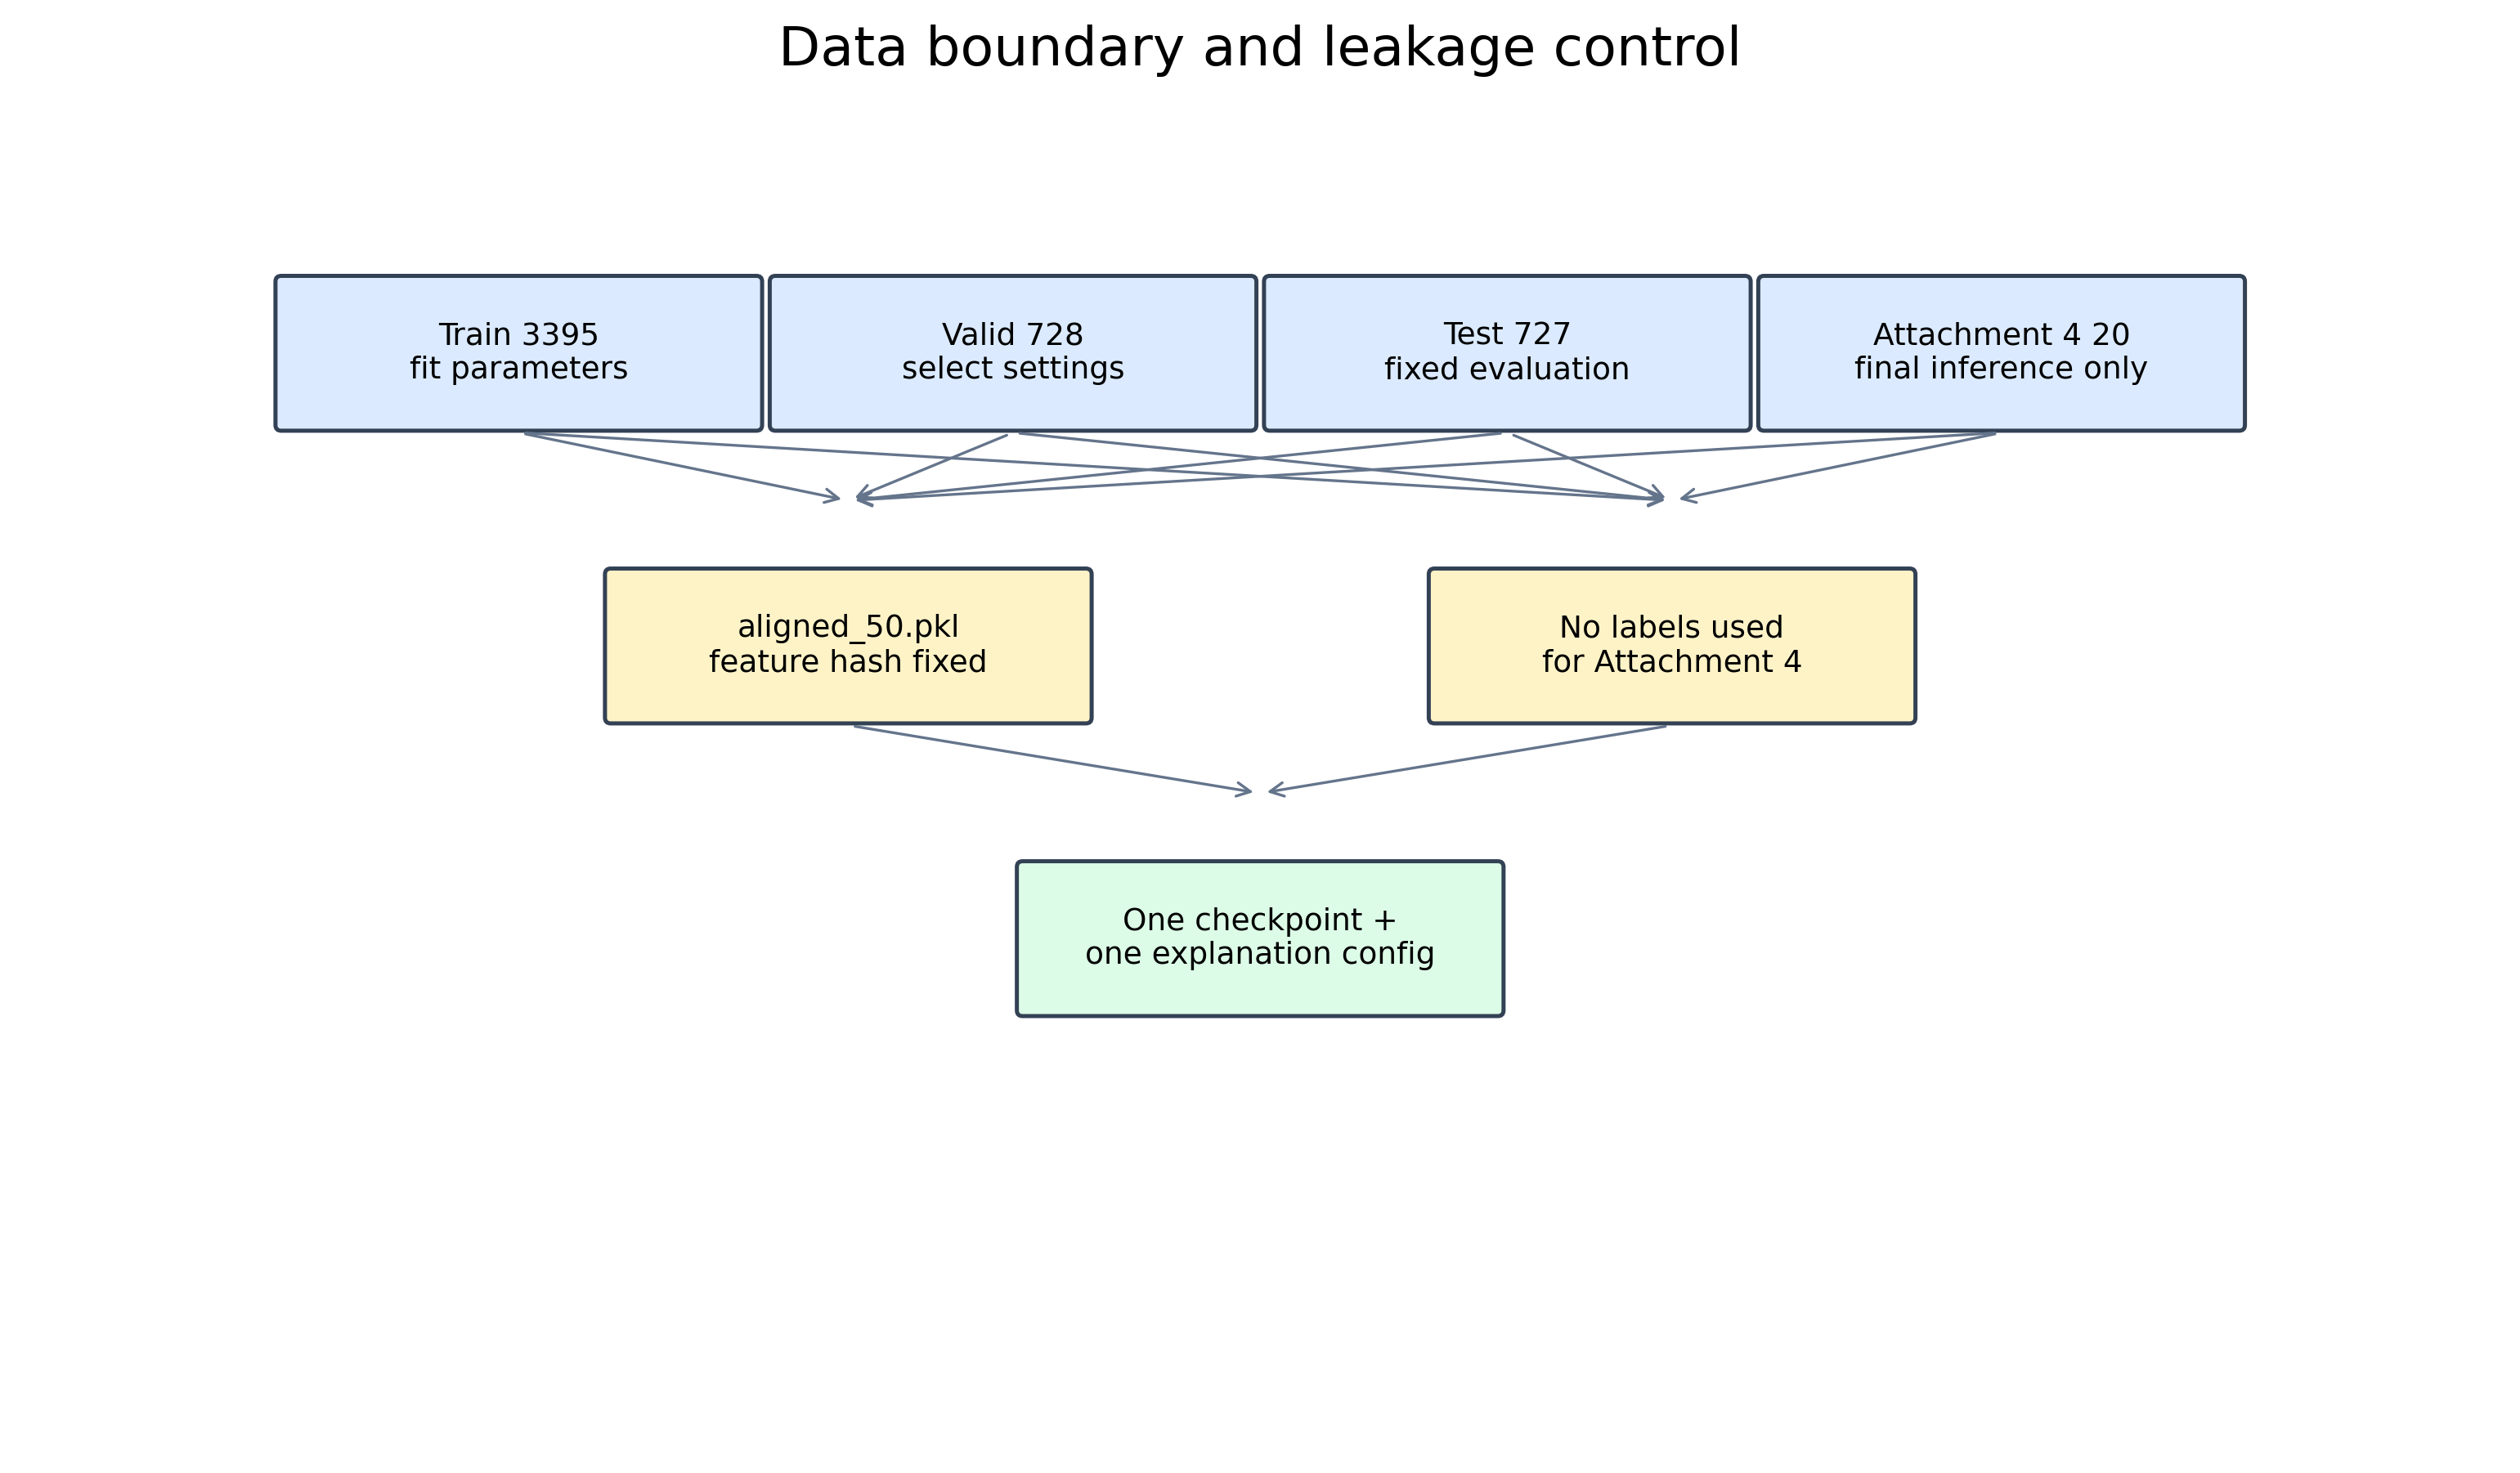
\includegraphics{assets/fig_data_boundary.png}
\caption{数据边界}\label{fig:boundary}
}
\end{figure}

图 2
给出数据边界。该边界是本文所有实验结果可解释性的前提：附件四预测不能写成
Accuracy、F1、MAE 或 Pearson。

\hypertarget{ux8f93ux5165ux8f93ux51faux5b9aux4e49}{%
\subsubsection{3.3
输入输出定义}\label{ux8f93ux5165ux8f93ux51faux5b9aux4e49}}

模型输入为三模态特征、三模态有效掩码、数据划分和样本主键。模型输出包括分类概率、预测类别、情感强度、门控值；解释模块进一步输出模态敏感性、归一化贡献、主要模态、局部窗口起止位置、相对时间、帧索引和映射状态。\texttt{predictions\_valid.csv}、\texttt{predictions\_test.csv}
和 \texttt{predictions\_attachment4.csv}
保存预测结果；\texttt{local\_importance\_*.csv}
保存局部遮挡影响；\texttt{evidence\_mapping\_*.csv} 保存证据回溯字段。

\hypertarget{ux591aux6a21ux6001ux9884ux6d4bux6a21ux578b}{%
\subsection{4
多模态预测模型}\label{ux591aux6a21ux6001ux9884ux6d4bux6a21ux578b}}

\hypertarget{ux6807ux51c6ux5316ux4e0eux6a21ux6001ux6295ux5f71}{%
\subsubsection{4.1
标准化与模态投影}\label{ux6807ux51c6ux5316ux4e0eux6a21ux6001ux6295ux5f71}}

设训练集统计量为 \(\mu_m\) 和 \(\sigma_m\)，仅对有效位置计算，则标准化为

\[
\widetilde{x}_{i,t}^{(m)}=\frac{x_{i,t}^{(m)}-\mu_m}{\max(\sigma_m,\varepsilon)}.
\tag{3}
\]

随后使用模态专属投影映射到统一隐空间：

\[
e_{i,t}^{(m)}=\operatorname{LN}(W_m\widetilde{x}_{i,t}^{(m)}+b_m),\quad e_{i,t}^{(m)}\in\mathbb R^{64}.
\tag{4}
\]

验证集、测试集和附件四均复用
\texttt{train\_standardizer.npz}，不重新估计均值和方差。

\hypertarget{ux63a9ux7801ux611fux77e5ux65f6ux5e8fux7f16ux7801}{%
\subsubsection{4.2
掩码感知时序编码}\label{ux63a9ux7801ux611fux77e5ux65f6ux5e8fux7f16ux7801}}

加入可学习位置表示 \(p_t\) 后，对每个模态使用独立 Transformer 编码器：

\[
\bar e_{i,t}^{(m)}=e_{i,t}^{(m)}+p_t,
\qquad H_i^{(m)}=\operatorname{Encoder}_m(\bar E_i^{(m)},M_i^{(m)}).
\tag{5}
\]

无效键位置在注意力中被屏蔽。编码结果采用掩码平均池化：

\[
g_i^{(m)}=\frac{\sum_{t=1}^{L_m}m_{i,t}^{(m)}H_{i,t}^{(m)}}{\max(1,\sum_{t=1}^{L_m}m_{i,t}^{(m)})}.
\tag{6}
\]

该处理保证 padding 不会被当作情感信息，并支持局部模态缺失。

\hypertarget{ux6587ux672cux5f15ux5bfcux7684ux8de8ux6a21ux6001ux4ea4ux4e92}{%
\subsubsection{4.3
文本引导的跨模态交互}\label{ux6587ux672cux5f15ux5bfcux7684ux8de8ux6a21ux6001ux4ea4ux4e92}}

以文本序列为查询，分别从音频和视觉中提取补充信息：

\[
R_i^{T\leftarrow A}=\operatorname{MHA}(H_i^{(T)},H_i^{(A)},H_i^{(A)};M_i^{(A)}),
\tag{7}
\]

\[
R_i^{T\leftarrow V}=\operatorname{MHA}(H_i^{(T)},H_i^{(V)},H_i^{(V)};M_i^{(V)}).
\tag{8}
\]

源码中两类跨模态响应按照文本有效位置池化后加到文本摘要，再与音频、视觉摘要组成门控输入：

\[
\widetilde g_i^{(T)}=g_i^{(T)}+\operatorname{Pool}(R_i^{T\leftarrow A})+\operatorname{Pool}(R_i^{T\leftarrow V}),
\quad G_i=[\widetilde g_i^{(T)};g_i^{(A)};g_i^{(V)}]^{\mathsf T}.
\tag{9}
\]

\begin{figure}
\hypertarget{fig:architecture}{%
\centering
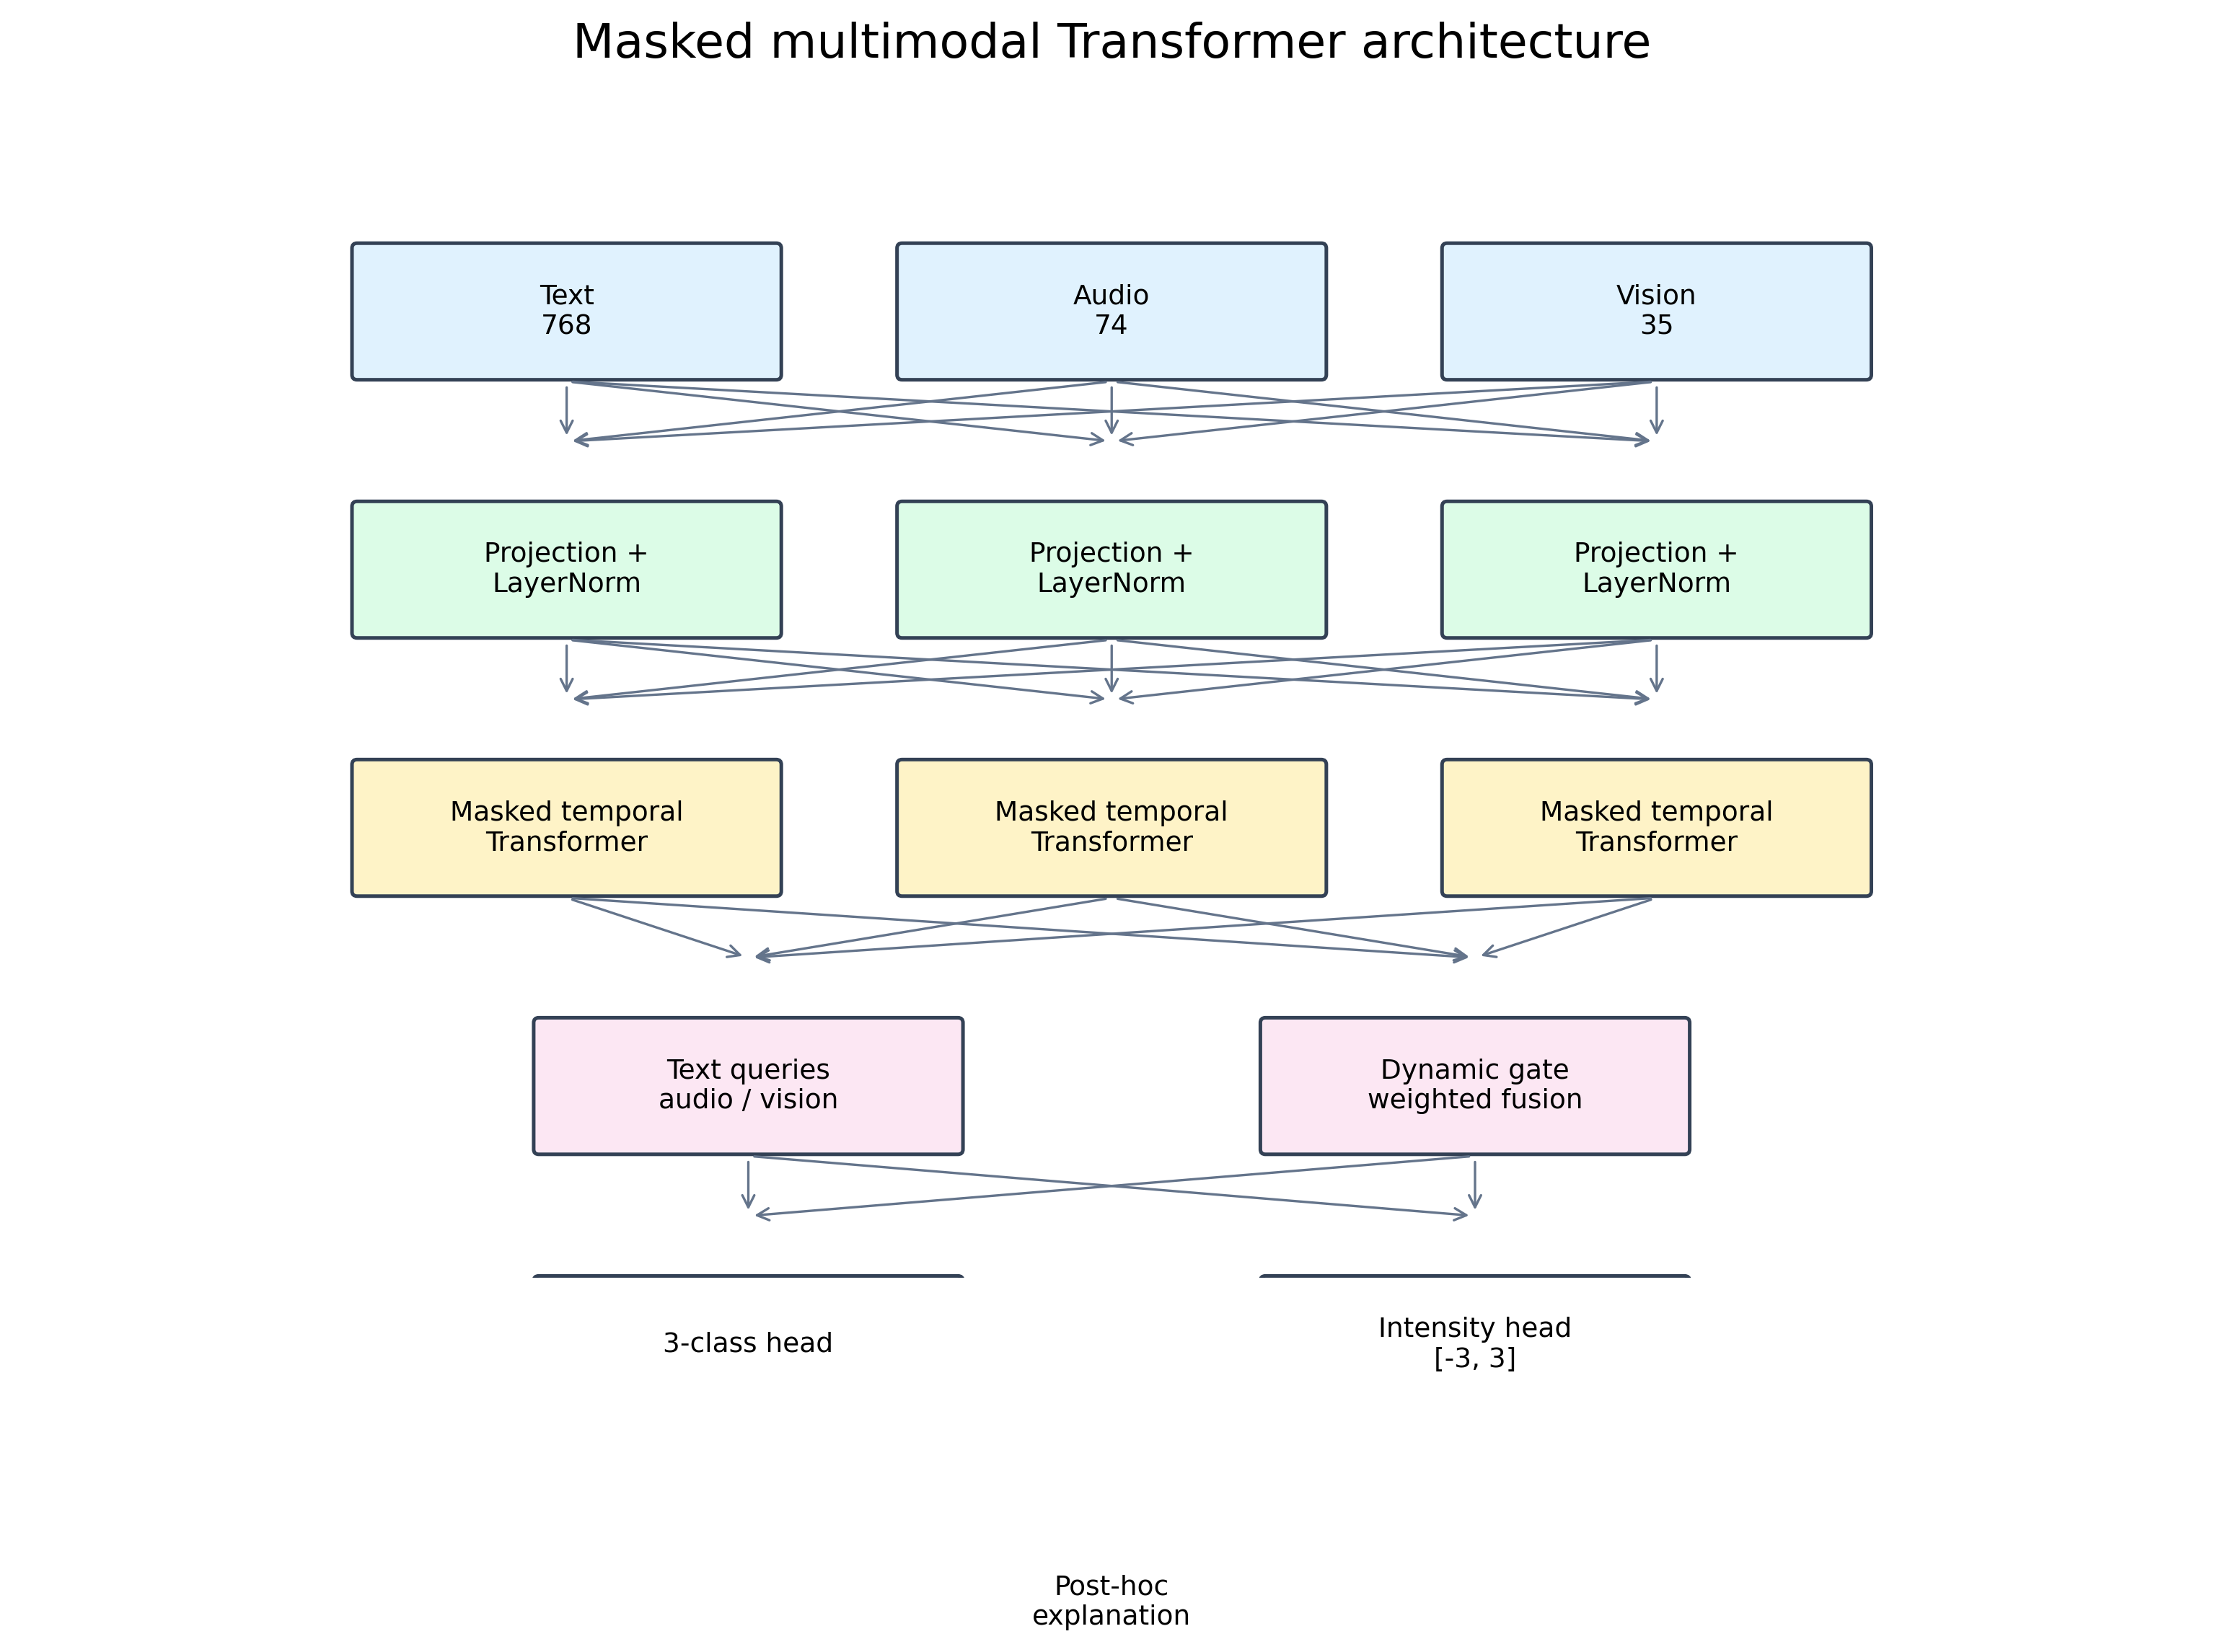
\includegraphics{assets/fig_model_architecture.png}
\caption{模型结构}\label{fig:architecture}
}
\end{figure}

图 3 展示实际模型结构。跨模态注意力用于表征增强，不直接作为最终解释。

\hypertarget{ux52a8ux6001ux95e8ux63a7ux4e0eux53ccux4efbux52a1ux8f93ux51fa}{%
\subsubsection{4.4
动态门控与双任务输出}\label{ux52a8ux6001ux95e8ux63a7ux4e0eux53ccux4efbux52a1ux8f93ux51fa}}

对每个样本和模态计算门控分数：

\[
a_i^{(m)}=w^{\mathsf T}G_{i,m}+b,qquad
\alpha_i^{(m)}=\frac{q_i^{(m)}e^{a_i^{(m)}}}{\sum_rq_i^{(r)}e^{a_i^{(r)}}+\varepsilon},
\tag{10}
\]

其中 \(q_i^{(m)}\) 表示模态是否存在有效观测。融合表示为

\[
z_i=\operatorname{MLP}\left(\sum_{m\in\{T,A,V\}}\alpha_i^{(m)}G_{i,m}\right).
\tag{11}
\]

分类概率和回归输出分别为

\[
p_i=\operatorname{softmax}(W_{cls}z_i+b_{cls}),
\tag{12}
\]

\[
\hat y_i=3\tanh(w_{reg}^{\mathsf T}z_i+b_{reg}).
\tag{13}
\]

联合目标函数为

\[
\mathcal L=\lambda_{cls}\mathcal L_{CE}+\lambda_{reg}\mathcal L_{SmoothL1},\qquad \lambda_{cls}=\lambda_{reg}=1.
\tag{14}
\]

\hypertarget{ux53cdux4e8bux5b9eux89e3ux91caux6a21ux578b}{%
\subsection{5
反事实解释模型}\label{ux53cdux4e8bux5b9eux89e3ux91caux6a21ux578b}}

\hypertarget{ux6a21ux6001ux8d21ux732e}{%
\subsubsection{5.1 模态贡献}\label{ux6a21ux6001ux8d21ux732e}}

固定预测模型后，对模态 \(m\) 使用训练集均值基线进行替换，得到
\((p_i^{-m},\hat y_i^{-m})\)。分类和回归变化分别为

\[
\Delta_{i,m}^{cls}=D_{KL}(p_i\Vert p_i^{-m}),\qquad \Delta_{i,m}^{reg}=|\hat y_i-\hat y_i^{-m}|.
\tag{15}
\]

在验证集预先固定尺度后定义综合敏感性 \(r_{i,m}\)，并归一化为

\[
c_{i,m}=\frac{\max(r_{i,m},0)}{\sum_{r\in\{T,A,V\}}\max(r_{i,r},0)+\varepsilon}.
\tag{16}
\]

\(c_{i,m}\) 之和约为
1，最大值对应主要模态。该值是模型后验敏感性，不是因果真值。

\hypertarget{ux5c40ux90e8ux8bc1ux636eux4e0eux5fe0ux5b9eux6027}{%
\subsubsection{5.2
局部证据与忠实性}\label{ux5c40ux90e8ux8bc1ux636eux4e0eux5fe0ux5b9eux6027}}

局部窗口长度和步长均为 7。对窗口内特征执行基线替换，计算

\[
r_{i,m,k}^{local}=\rho D_{KL}(p_i\Vert p_i^{-m,k})+(1-\rho)|\hat y_i-\hat y_i^{-m,k}|.
\tag{17}
\]

每个样本保留 Top-3 窗口。验证集 728 个样本中，高重要性窗口平均影响为
0.0748529，低重要性窗口为 0.0032877，差值为 0.0715652，比例为
22.7675。该结果支持窗口排序具有模型敏感性区分能力。

\begin{figure}
\hypertarget{fig:fidelity}{%
\centering
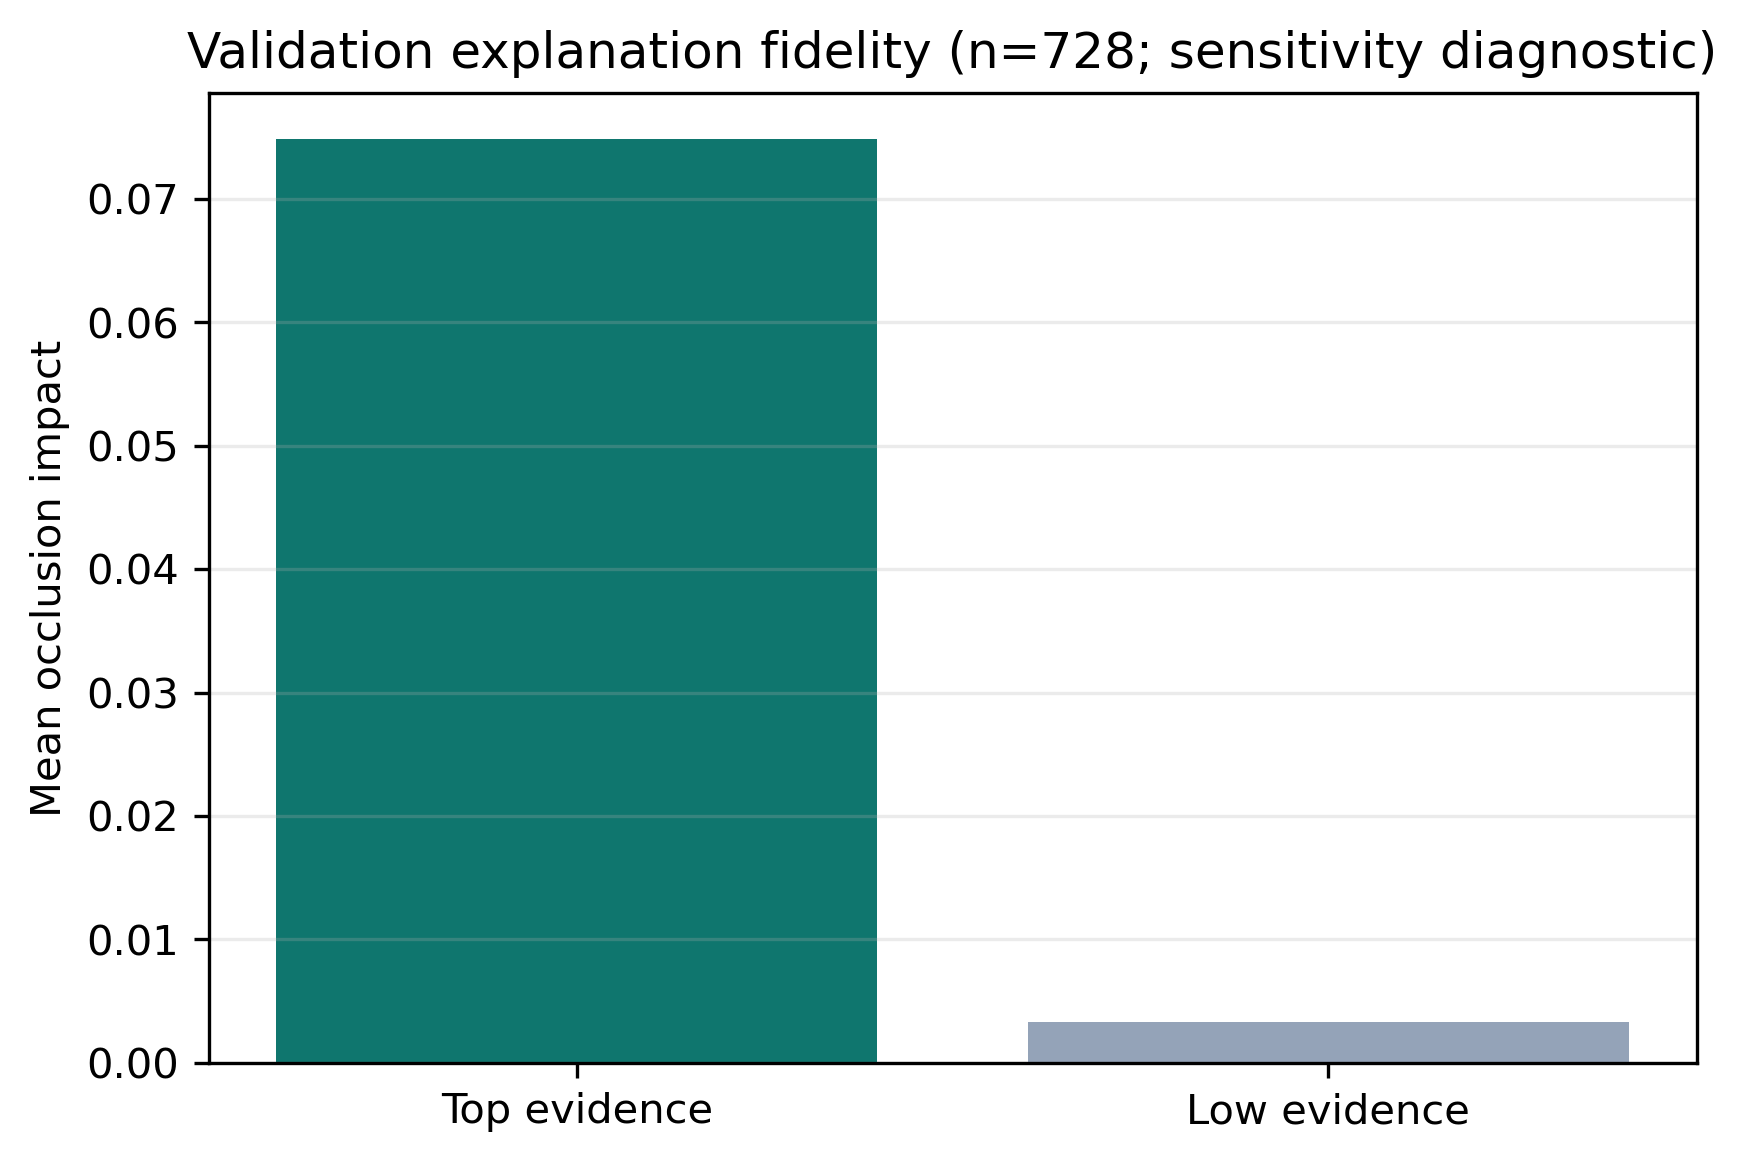
\includegraphics{assets/fig_fidelity_valid.png}
\caption{验证集解释忠实性}\label{fig:fidelity}
}
\end{figure}

图 4
是验证集忠实性诊断；它验证的是遮挡排序与模型输出变化的一致性，不是人工证据准确率。

\hypertarget{ux5b9eux9a8cux8bbeux7f6eux4e0eux8bc4ux4ef7ux6307ux6807}{%
\subsection{6
实验设置与评价指标}\label{ux5b9eux9a8cux8bbeux7f6eux4e0eux8bc4ux4ef7ux6307ux6807}}

\hypertarget{ux5b9eux9a8cux914dux7f6e}{%
\subsubsection{6.1 实验配置}\label{ux5b9eux9a8cux914dux7f6e}}

\begin{longtable}[]{@{}ll@{}}
\toprule
参数 & 实际设置 \\
\midrule
\endhead
特征版本 & aligned\_50，长度 50 \\
输入维度 & 768 / 74 / 35 \\
隐空间、层数、头数 & 64 / 1 / 4 \\
Dropout & 0.1 \\
Batch size、Epoch & 64 / 50 \\
学习率、权重衰减 & \(2\times10^{-5}\) / \(1\times10^{-4}\) \\
随机种子、设备 & 20260924 / CUDA \\
解释基线 & train\_mean，标准化训练特征空间 \\
窗口、步长、Top-K & 7 / 7 / 3 \\
\bottomrule
\end{longtable}

训练曲线来自 \texttt{training\_curve.csv}，模型在第 29 个 epoch
获得最低验证损失 1.1744457，最终保留该最佳 epoch 对应权重。

\begin{figure}
\hypertarget{fig:training}{%
\centering
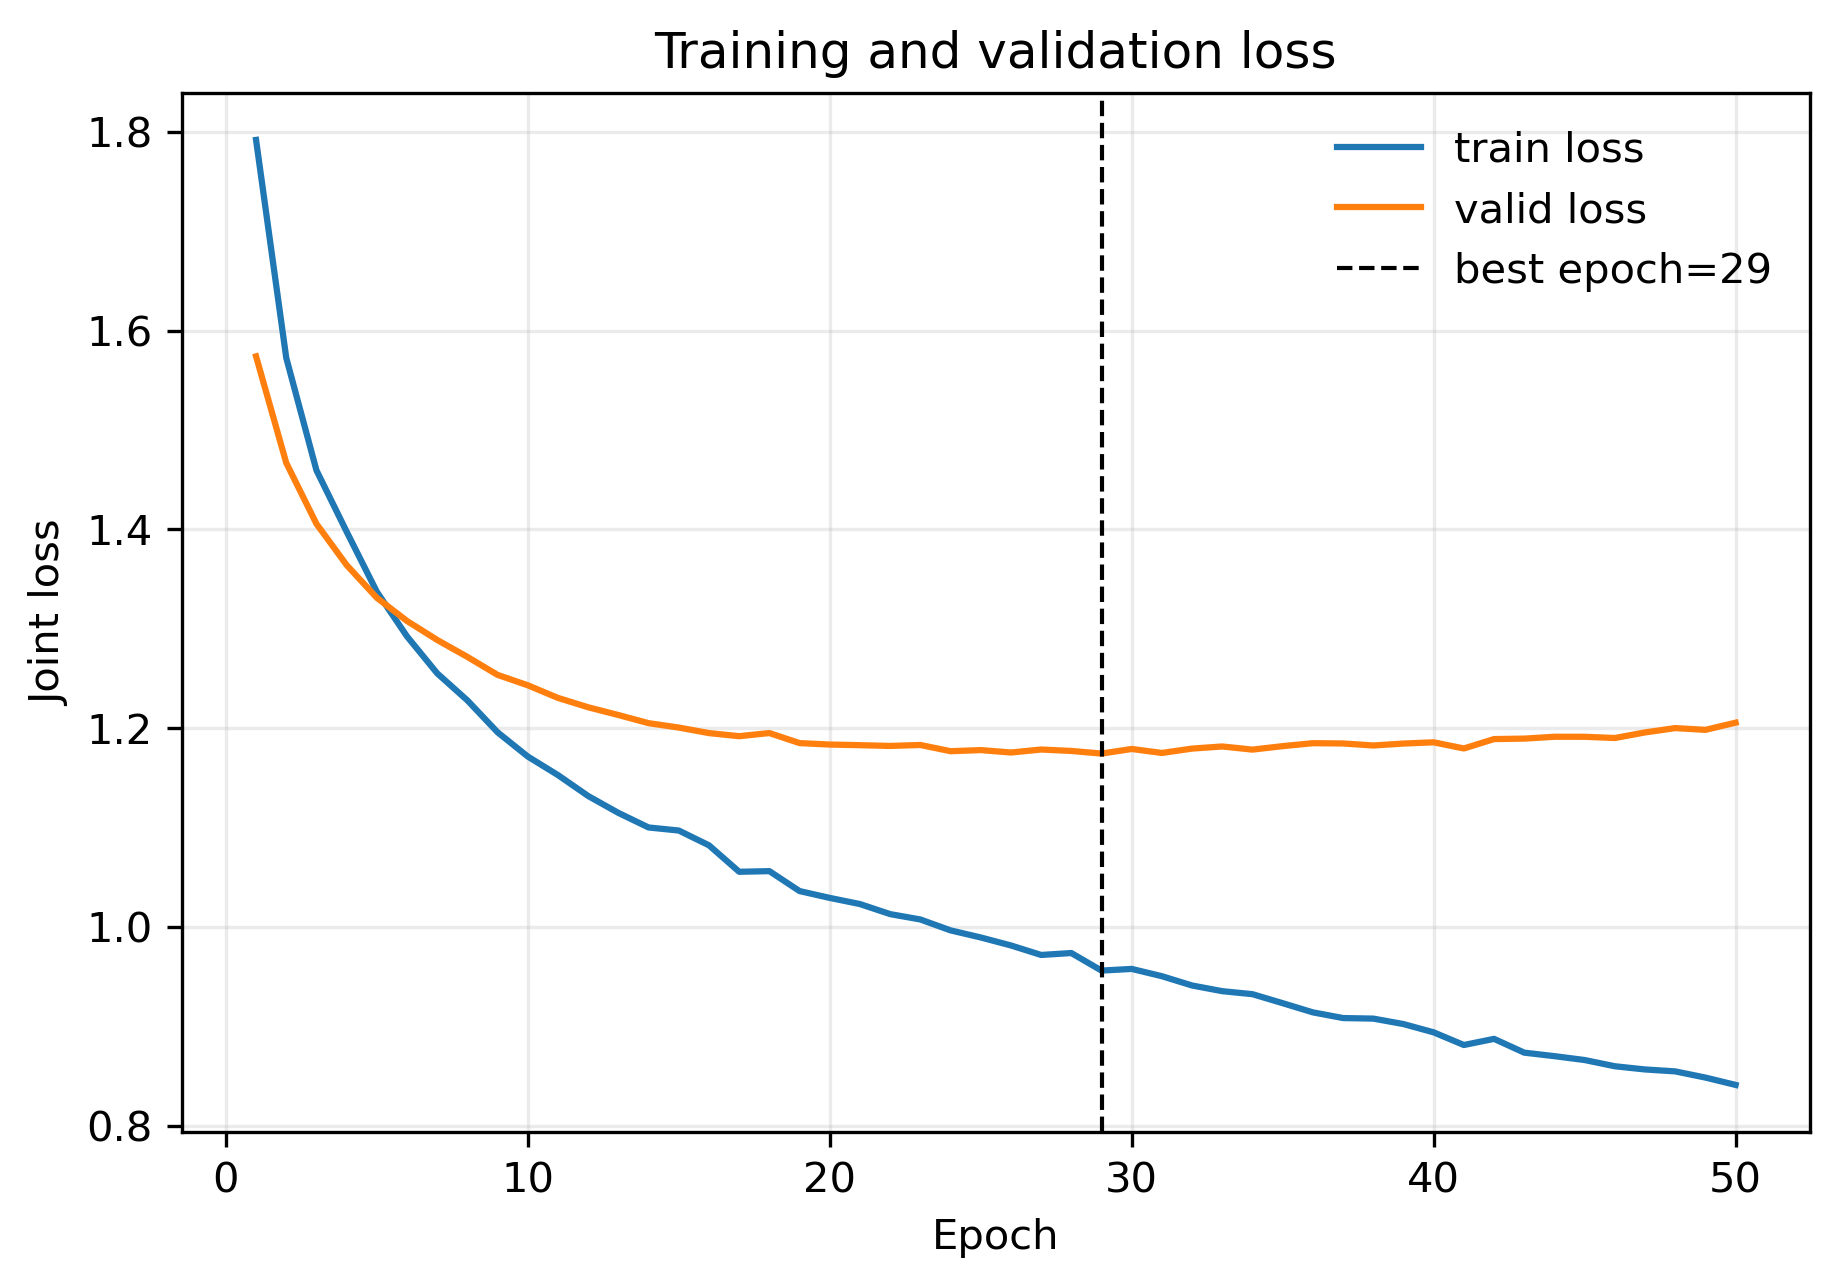
\includegraphics{assets/fig_training_curve.png}
\caption{训练曲线}\label{fig:training}
}
\end{figure}

图 5 与训练日志共同表明，训练损失从第 1 个 epoch 的 1.7918299 降至第 50
个 epoch 的 0.8410989；验证损失在第 29 个 epoch 达到
1.1744457，之后未继续改善，模型选择遵循验证集而非测试集。

\hypertarget{ux8bc4ux4ef7ux6307ux6807}{%
\subsubsection{6.2 评价指标}\label{ux8bc4ux4ef7ux6307ux6807}}

分类采用 Accuracy 与 Macro-F1，回归采用 MAE 与 Pearson：

\[
Accuracy=\frac{1}{N}\sum_i\mathbf 1(\hat c_i=c_i),\qquad Macro\text{-}F1=\frac{1}{3}\sum_{c=0}^2F1_c.
\tag{18}
\]

\[
MAE=\frac{1}{N}\sum_i|\hat y_i-y_i|,
\tag{19}
\]

\[
Pearson=\frac{\sum_i(\hat y_i-\bar{\hat y})(y_i-\bar y)}{\sqrt{\sum_i(\hat y_i-\bar{\hat y})^2}\sqrt{\sum_i(y_i-\bar y)^2}}.
\tag{20}
\]

\hypertarget{ux6709ux6807ux7b7eux5b9eux9a8cux7ed3ux679c}{%
\subsection{7
有标签实验结果}\label{ux6709ux6807ux7b7eux5b9eux9a8cux7ed3ux679c}}

\hypertarget{ux603bux4f53ux6027ux80fd}{%
\subsubsection{7.1 总体性能}\label{ux603bux4f53ux6027ux80fd}}

表 1 直接对应 \texttt{model\_metrics.csv}。

\textbf{表 1 双任务模型总体性能}

\begin{longtable}[]{@{}lrrrr@{}}
\toprule
划分 & Accuracy & Macro-F1 & MAE & Pearson \\
\midrule
\endhead
valid（728） & 0.607143 & 0.547565 & 0.652097 & 0.580993 \\
test（727） & 0.672627 & 0.595023 & 0.679413 & 0.625911 \\
\bottomrule
\end{longtable}

\begin{figure}
\hypertarget{fig:cmvalid}{%
\centering

\includegraphics{assets/fig_confusion_matrix_valid.png}
\caption{验证集混淆矩阵}\label{fig:cmvalid}
}
\end{figure}

\begin{figure}
\hypertarget{fig:cmtest}{%
\centering
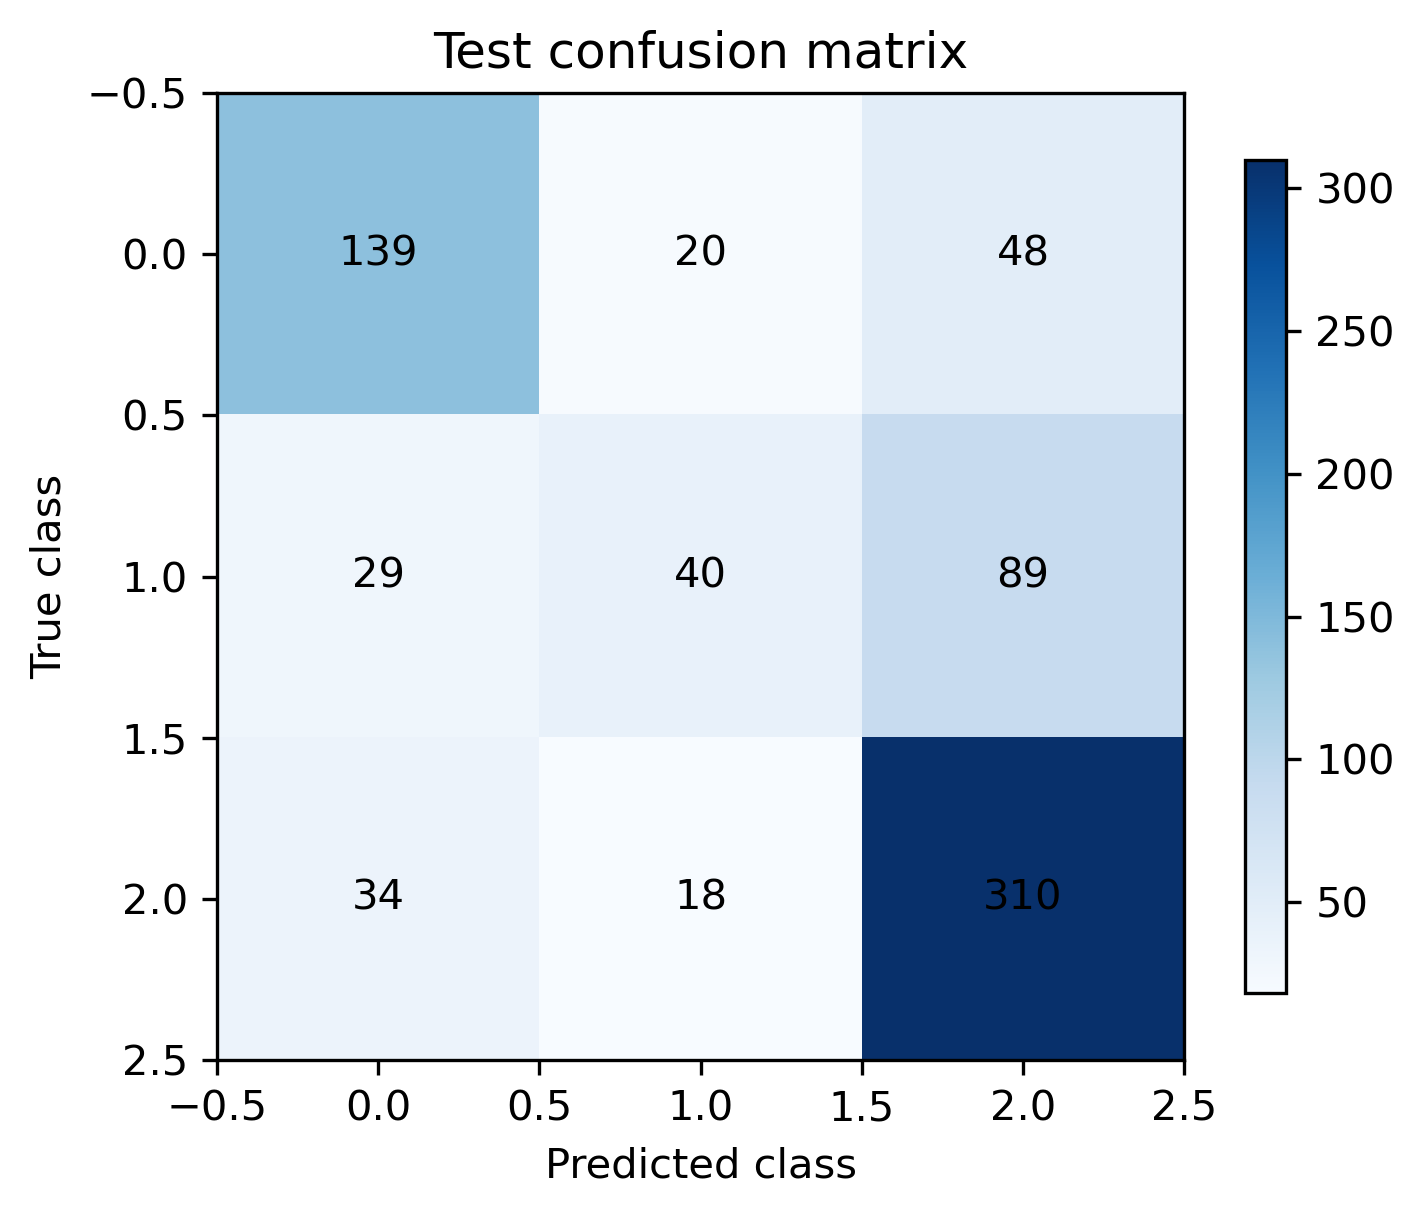
\includegraphics{assets/fig_confusion_matrix_test.png}
\caption{测试集混淆矩阵}\label{fig:cmtest}
}
\end{figure}

图 6 和图 7 展示分类混淆结构。test Accuracy 为 0.672627、Macro-F1 为
0.595023；回归 MAE 为 0.679413，Pearson 为
0.625911。当前只使用一个随机种子，因此不报告显著性或多种子置信区间。

\hypertarget{ux7c7bux522bux7ea7ux7ed3ux679c}{%
\subsubsection{7.2 类别级结果}\label{ux7c7bux522bux7ea7ux7ed3ux679c}}

\textbf{表 2 验证集分类报告}

\begin{longtable}[]{@{}lrrrr@{}}
\toprule
类别 & Precision & Recall & F1 & Support \\
\midrule
\endhead
Negative & 0.6465 & 0.6214 & 0.6337 & 206 \\
Neutral & 0.4433 & 0.2337 & 0.3060 & 184 \\
Positive & 0.6259 & 0.8018 & 0.7030 & 338 \\
\bottomrule
\end{longtable}

表 2 来自 \texttt{classification\_report\_valid.csv}。Positive
类召回率最高，而 Neutral 类召回率仅为
0.2337，说明中性样本容易被划入相邻极性类别。该现象仅作为当前运行的误差结构，不在缺少重训练对照的条件下归因于某个单一机制。

\begin{figure}
\hypertarget{fig:regvalid}{%
\centering
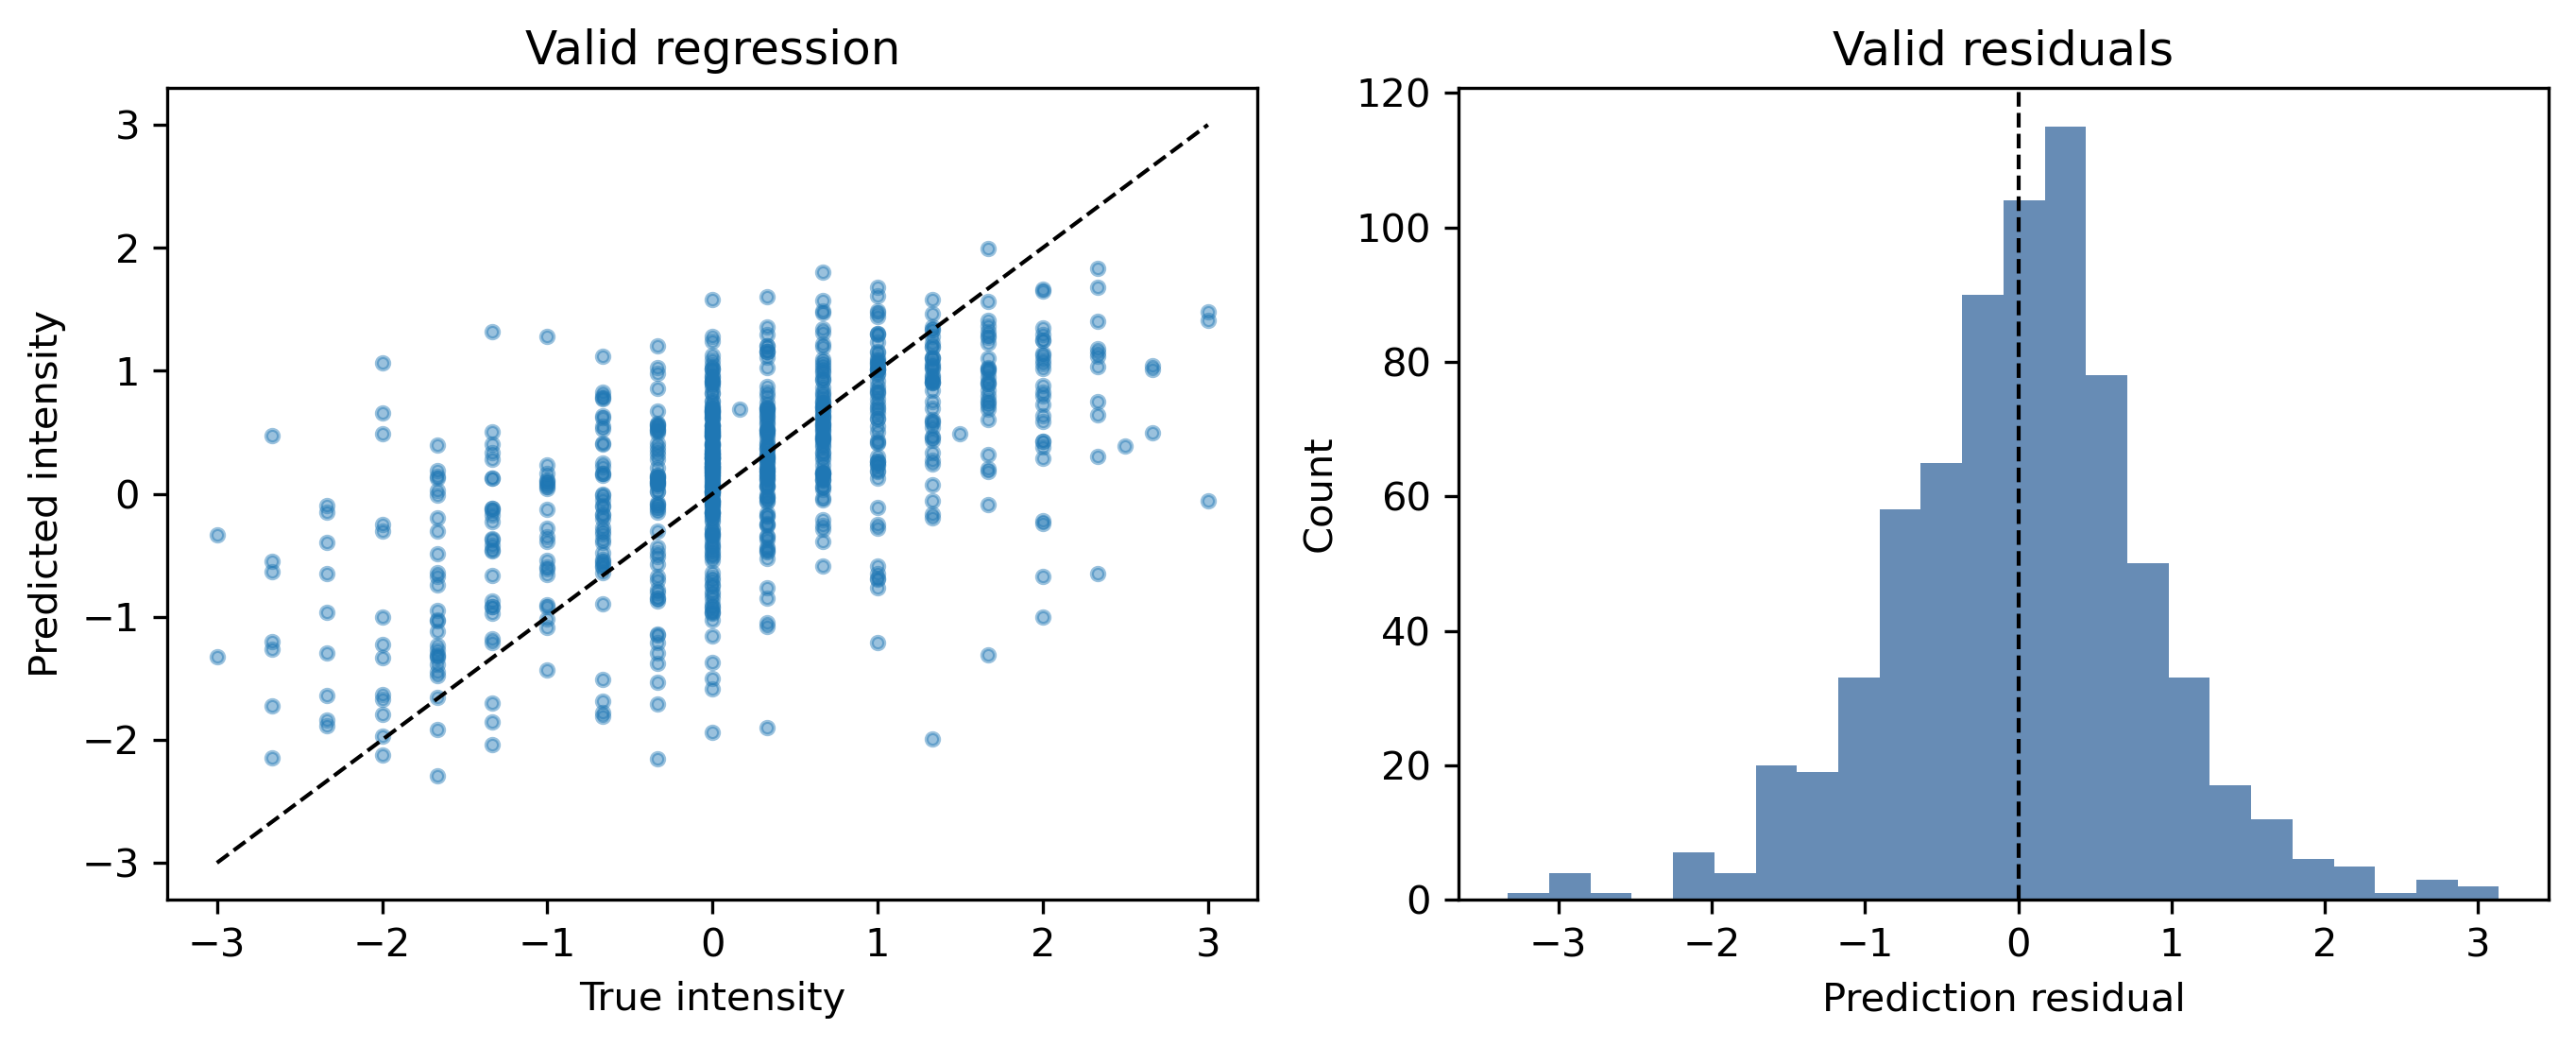
\includegraphics{assets/fig_regression_diagnostics_valid.png}
\caption{验证集回归诊断}\label{fig:regvalid}
}
\end{figure}

\begin{figure}
\hypertarget{fig:regtest}{%
\centering
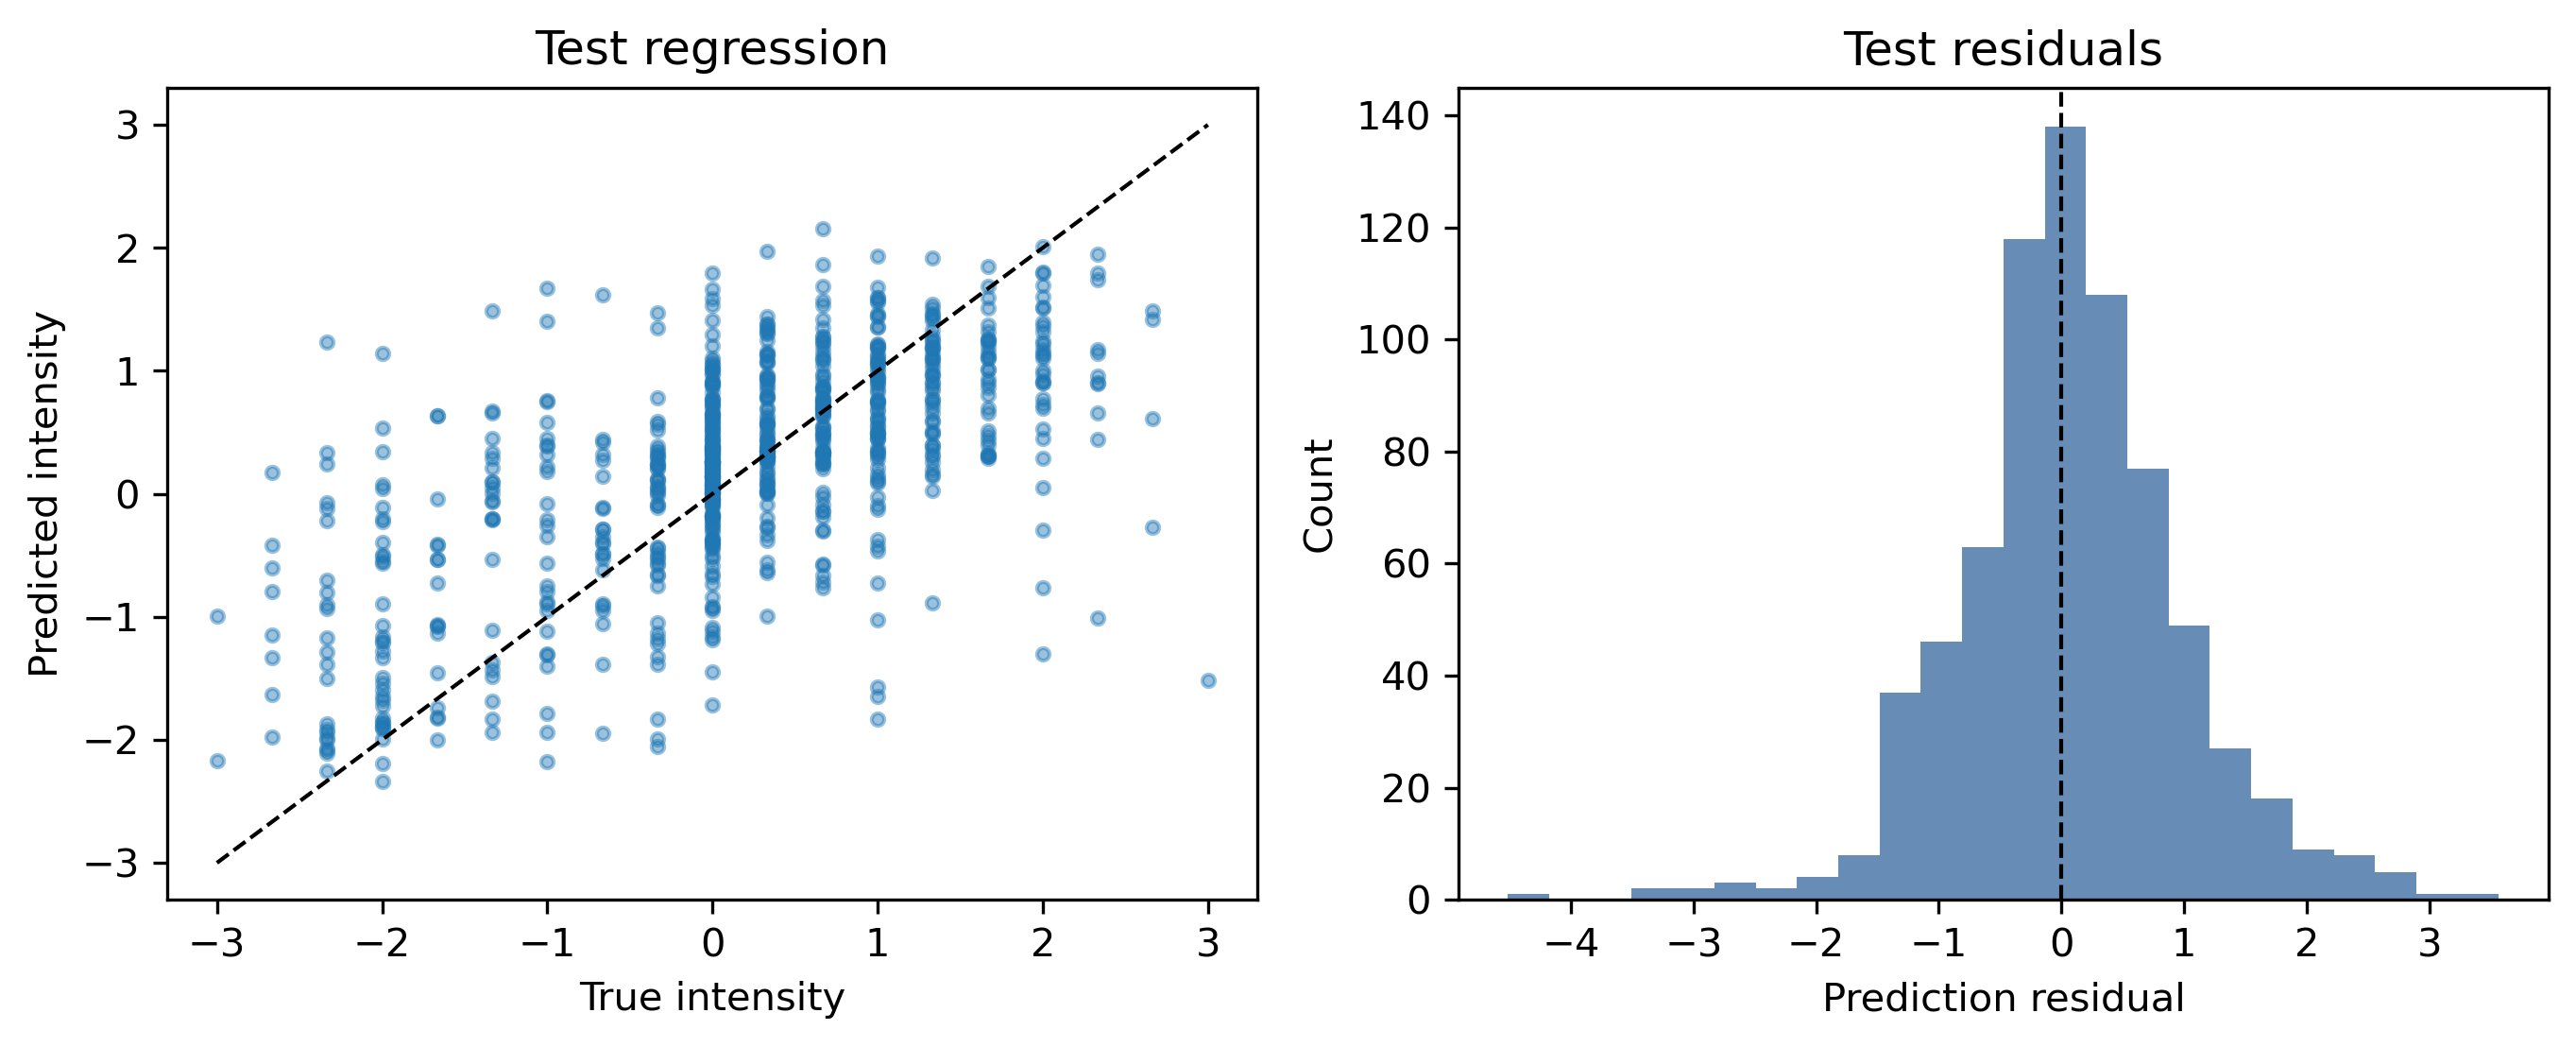
\includegraphics{assets/fig_regression_diagnostics_test.png}
\caption{测试集回归诊断}\label{fig:regtest}
}
\end{figure}

图 8 和图 9
是实际生成的回归诊断图，用于观察连续强度的预测偏差与离散程度，不能替代表
1 的 MAE 和 Pearson。

\hypertarget{ux6a21ux6001ux8d21ux732eux4e0eux540eux9a8cux8bcaux65ad}{%
\subsection{8
模态贡献与后验诊断}\label{ux6a21ux6001ux8d21ux732eux4e0eux540eux9a8cux8bcaux65ad}}

\hypertarget{ux5168ux5c40ux6a21ux6001ux8d21ux732e}{%
\subsubsection{8.1
全局模态贡献}\label{ux5168ux5c40ux6a21ux6001ux8d21ux732e}}

\textbf{表 3 反事实模态贡献统计}

\begin{longtable}[]{@{}llrrrr@{}}
\toprule
划分 & 模态 & 样本数 & 平均贡献 & 标准差 & 中位数 \\
\midrule
\endhead
valid & text & 728 & 0.564601 & 0.207986 & 0.583357 \\
valid & audio & 728 & 0.241857 & 0.153316 & 0.225415 \\
valid & vision & 728 & 0.193542 & 0.126525 & 0.178919 \\
test & text & 727 & 0.571946 & 0.207630 & 0.596444 \\
test & audio & 727 & 0.245046 & 0.152818 & 0.225407 \\
test & vision & 727 & 0.183009 & 0.128257 & 0.167823 \\
attachment4 & text & 20 & 0.641696 & 0.186134 & 0.716467 \\
attachment4 & audio & 20 & 0.197818 & 0.136718 & 0.166865 \\
attachment4 & vision & 20 & 0.160485 & 0.115804 & 0.142188 \\
\bottomrule
\end{longtable}

表 3 来自 \texttt{modality\_contribution\_summary.csv}；附件四三行是 20
个无标签样本的模态贡献统计，原始样本记录在
\texttt{predictions\_attachment4.csv}。有标签数据中，文本平均贡献约
0.565--0.572，音频约 0.242--0.245，视觉约
0.183--0.194。该结果表示当前模型对文本输入更敏感，不表示文本在真实情感形成中必然最重要。

\begin{figure}
\hypertarget{fig:global}{%
\centering
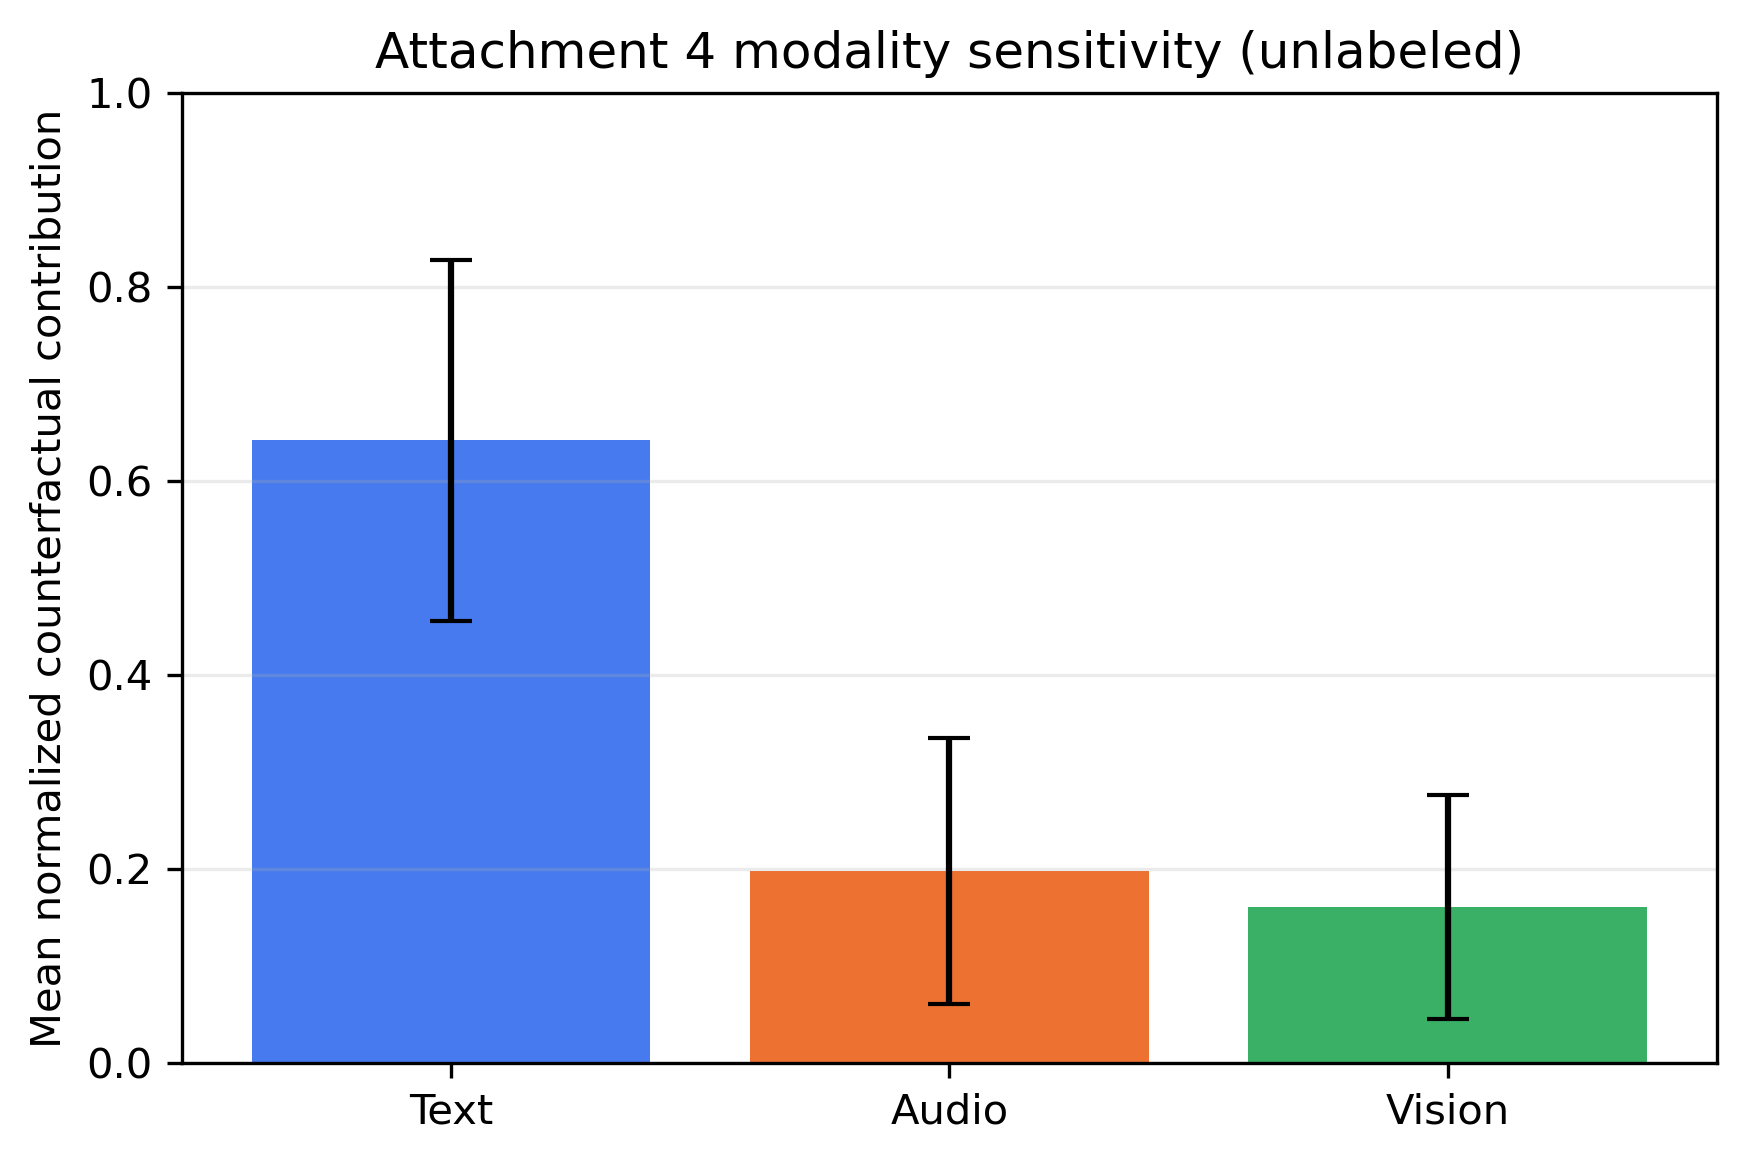
\includegraphics{assets/fig_global_contribution.png}
\caption{全局贡献}\label{fig:global}
}
\end{figure}

\begin{figure}
\hypertarget{fig:modalvalid}{%
\centering

\includegraphics{assets/fig_modality_contribution_valid.png}
\caption{验证集模态贡献}\label{fig:modalvalid}
}
\end{figure}

图 10 和图 11
分别展示全局贡献及验证集贡献分布。三类贡献均来自遮挡后输出变化，而不是直接读取门控值。

\hypertarget{ux6a21ux6001ux79fbux9664ux8bcaux65ad}{%
\subsubsection{8.2
模态移除诊断}\label{ux6a21ux6001ux79fbux9664ux8bcaux65ad}}

\textbf{表 4 固定模型的后验模态移除结果}

\begin{longtable}[]{@{}llrrrr@{}}
\toprule
划分 & 移除模态 & Accuracy & Macro-F1 & MAE & Pearson \\
\midrule
\endhead
valid & none & 0.607143 & 0.547565 & 0.652097 & 0.580993 \\
valid & text & 0.287088 & 0.263764 & 0.869413 & -0.020699 \\
valid & audio & 0.604396 & 0.571687 & 0.716655 & 0.579688 \\
valid & vision & 0.629121 & 0.576199 & 0.694256 & 0.573931 \\
test & none & 0.672627 & 0.595023 & 0.679413 & 0.625911 \\
test & text & 0.288858 & 0.266980 & 0.989222 & -0.064822 \\
test & audio & 0.678129 & 0.625366 & 0.733368 & 0.638242 \\
test & vision & 0.672627 & 0.592638 & 0.725985 & 0.613138 \\
\bottomrule
\end{longtable}

表 4 直接来自
\texttt{modality\_ablation\_metrics.csv}，是固定模型的后验模态移除诊断，不是重新训练的单模态基线。移除文本后
valid Accuracy 降至 0.287088、test Accuracy 降至 0.288858，且 Pearson
分别降至 -0.020699 和
-0.064822，说明模型预测对文本输入高度敏感；音频、视觉移除后的分类变化较小，但回归误差上升，说明二者仍可能提供补充强度信息。

\begin{figure}
\hypertarget{fig:gate}{%
\centering
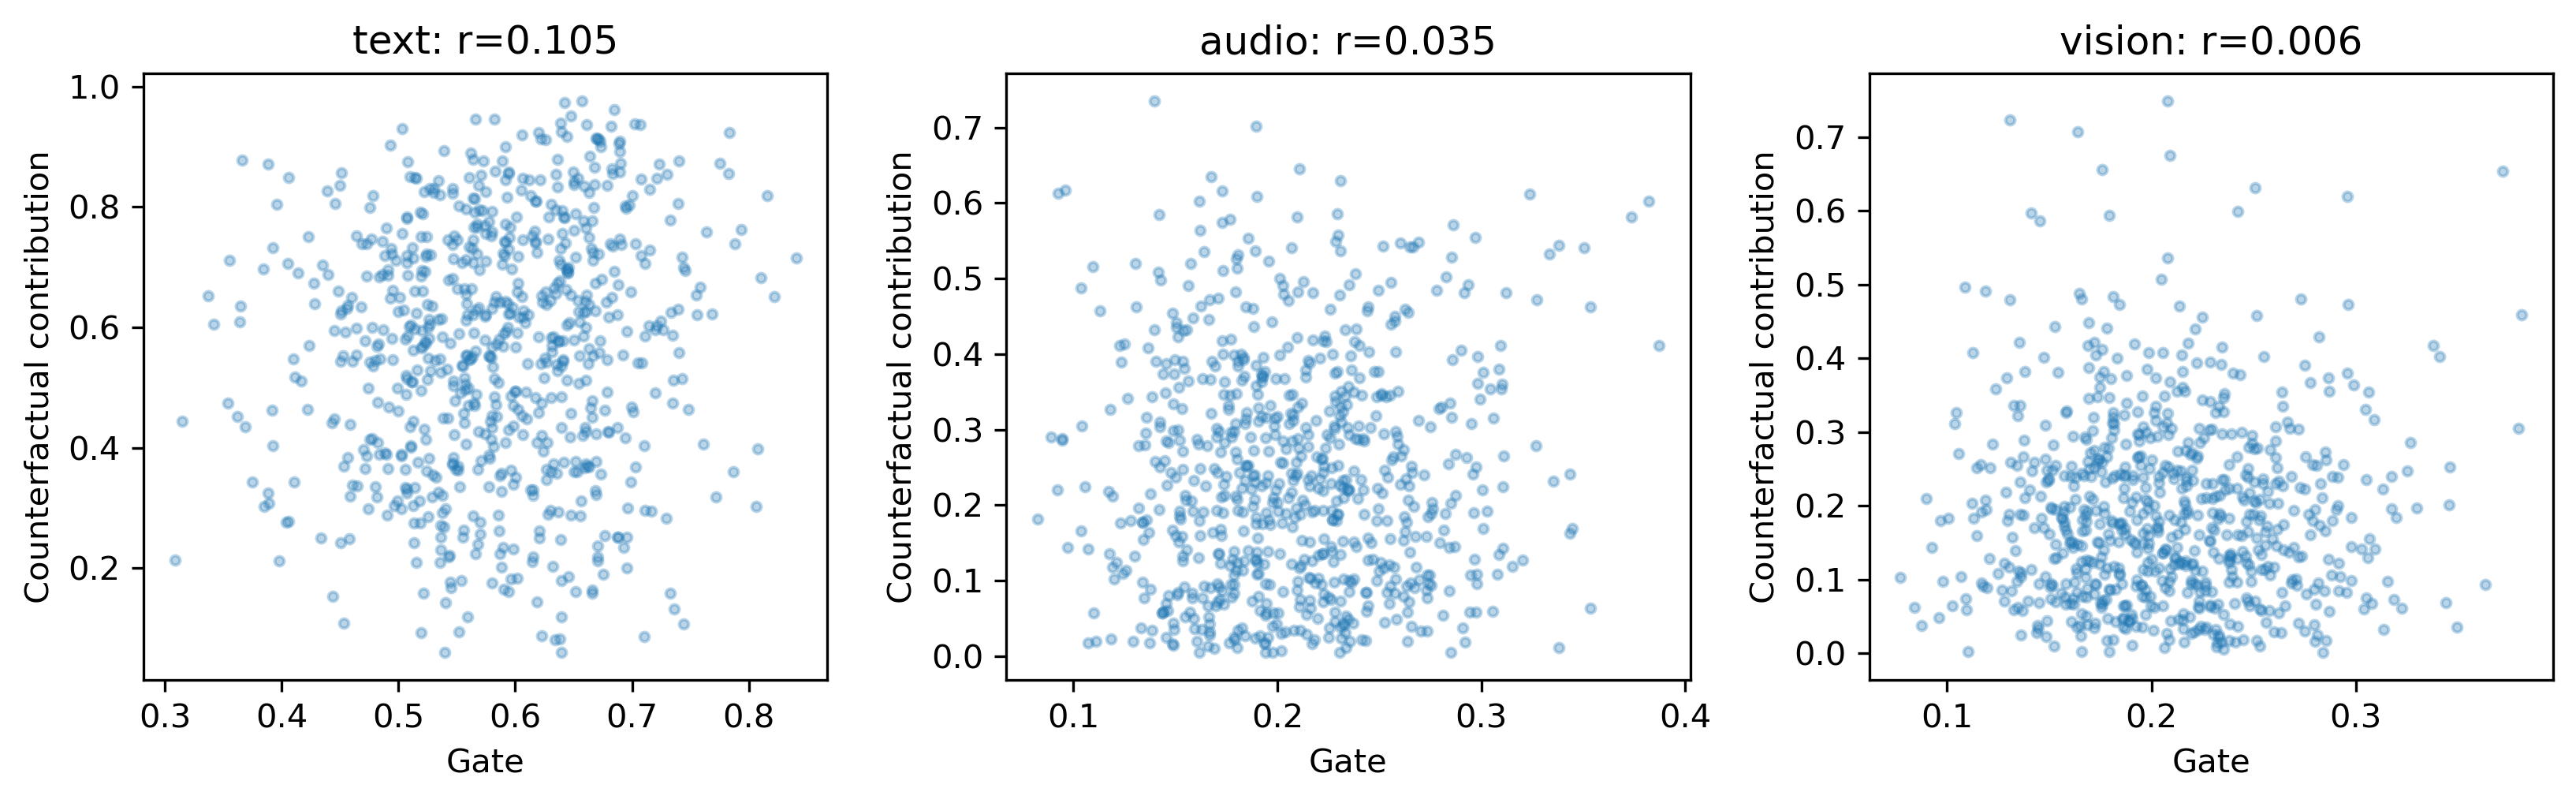
\includegraphics{assets/fig_gate_vs_contribution_valid.png}
\caption{门控与反事实贡献}\label{fig:gate}
}
\end{figure}

\begin{figure}
\hypertarget{fig:mapping}{%
\centering
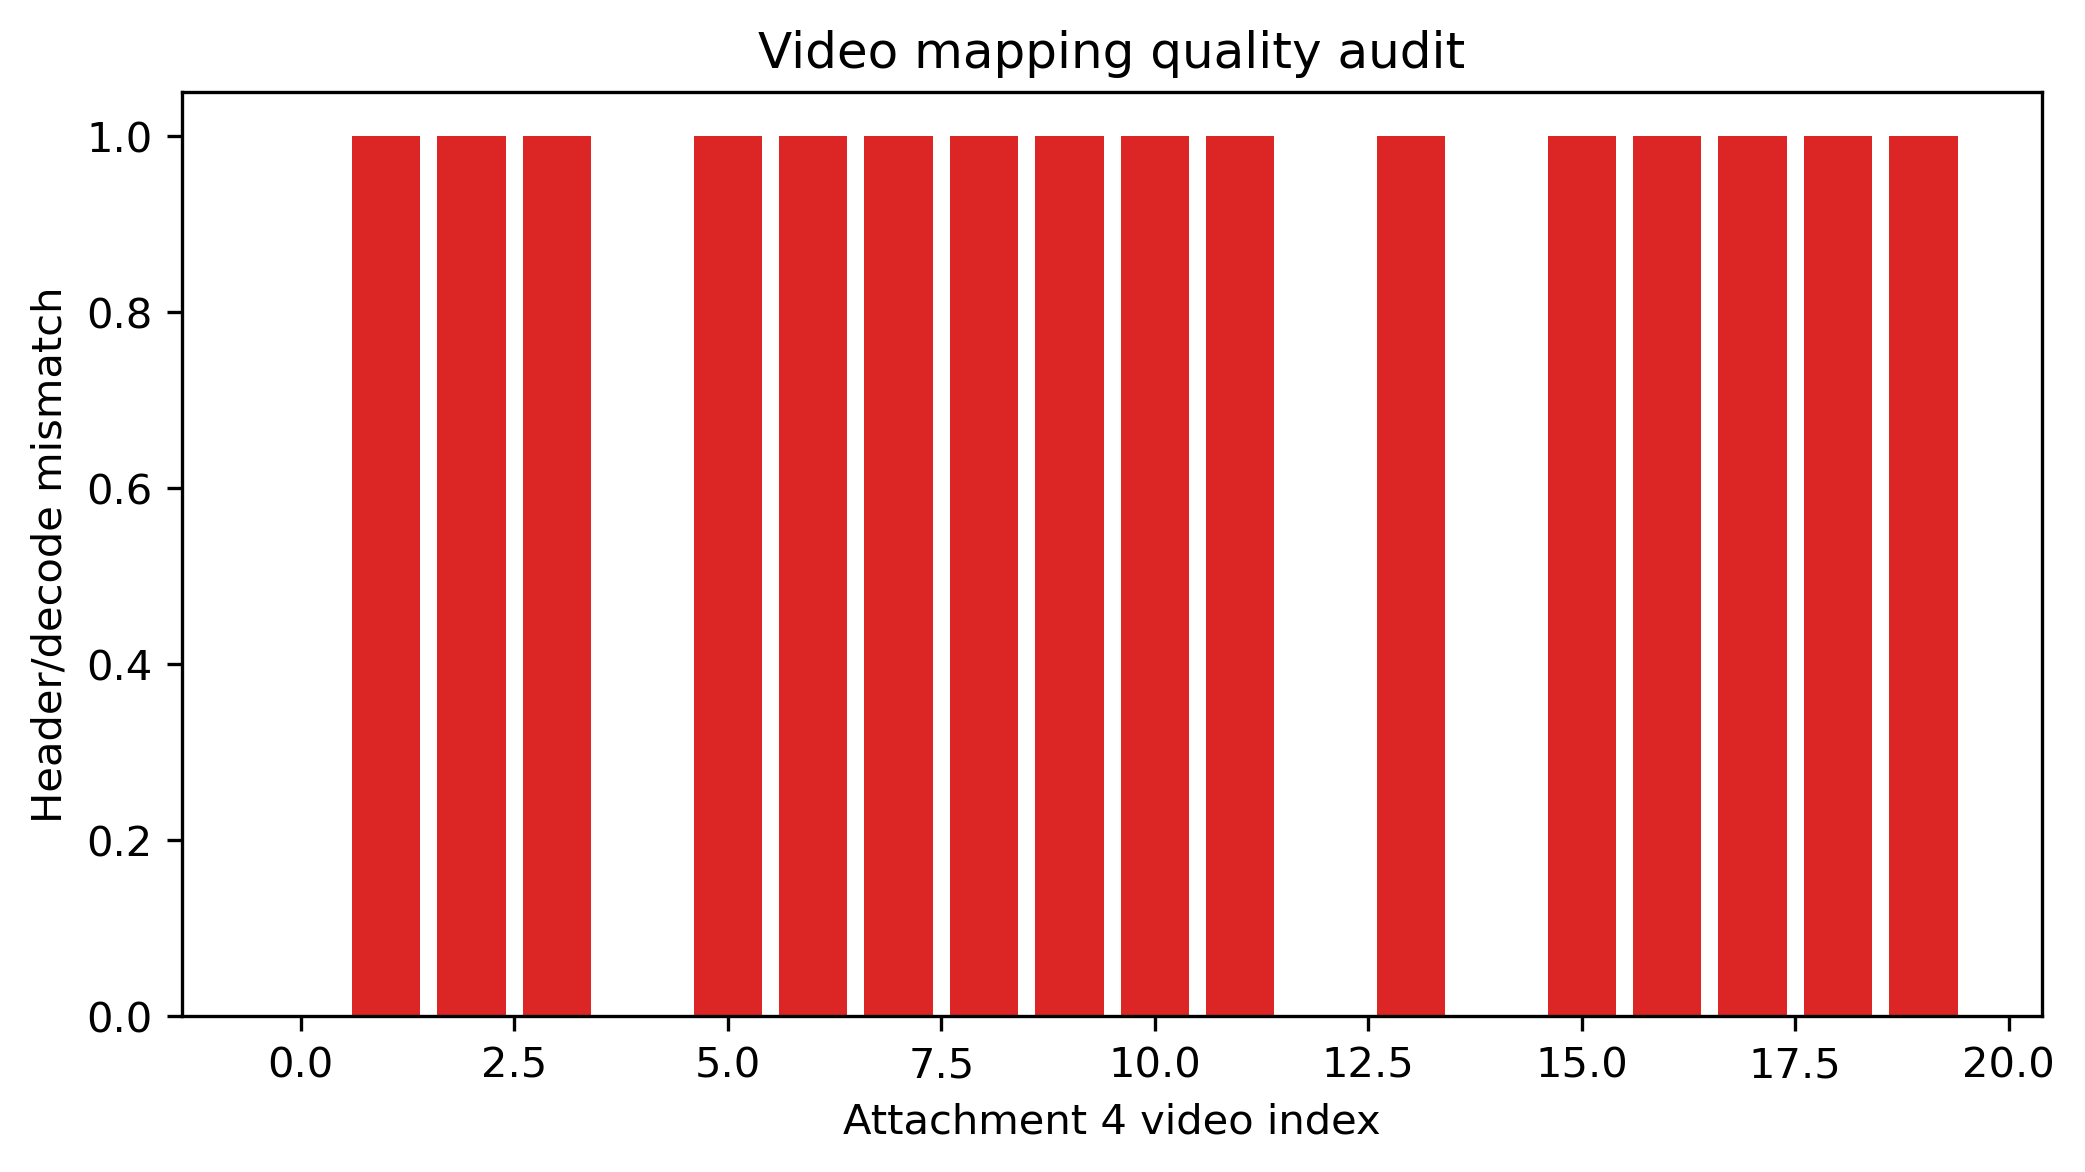
\includegraphics{assets/fig_mapping_quality.png}
\caption{门控一致性}\label{fig:mapping}
}
\end{figure}

图 12
展示门控值与反事实贡献的关系。\texttt{gate\_contribution\_consistency.csv}
给出的 Pearson 相关系数为 text 0.1050、audio 0.0349、vision
0.0061，相关性较弱，进一步说明门控值不能替代反事实贡献。图 13
展示映射质量统计，所有附件四证据行均完成边界检查，未发生证据行被截断。

\hypertarget{ux5c40ux90e8ux8bc1ux636eux5173ux952eux5e27ux4e0eux9644ux4ef6ux56dbux7ed3ux679c}{%
\subsection{9
局部证据、关键帧与附件四结果}\label{ux5c40ux90e8ux8bc1ux636eux5173ux952eux5e27ux4e0eux9644ux4ef6ux56dbux7ed3ux679c}}

\hypertarget{ux5c40ux90e8ux91cdux8981ux6027}{%
\subsubsection{9.1 局部重要性}\label{ux5c40ux90e8ux91cdux8981ux6027}}

\texttt{local\_importance\_valid.csv}、\texttt{local\_importance\_test.csv}
和 \texttt{local\_importance\_attachment4.csv}
分别保存三种划分的窗口影响；图 14--16 展示相应热力图。valid 和 test
热力图可结合真实标签分析证据与误差，附件四热力图只用于推理证据展示。

\begin{figure}
\hypertarget{fig:localvalid}{%
\centering
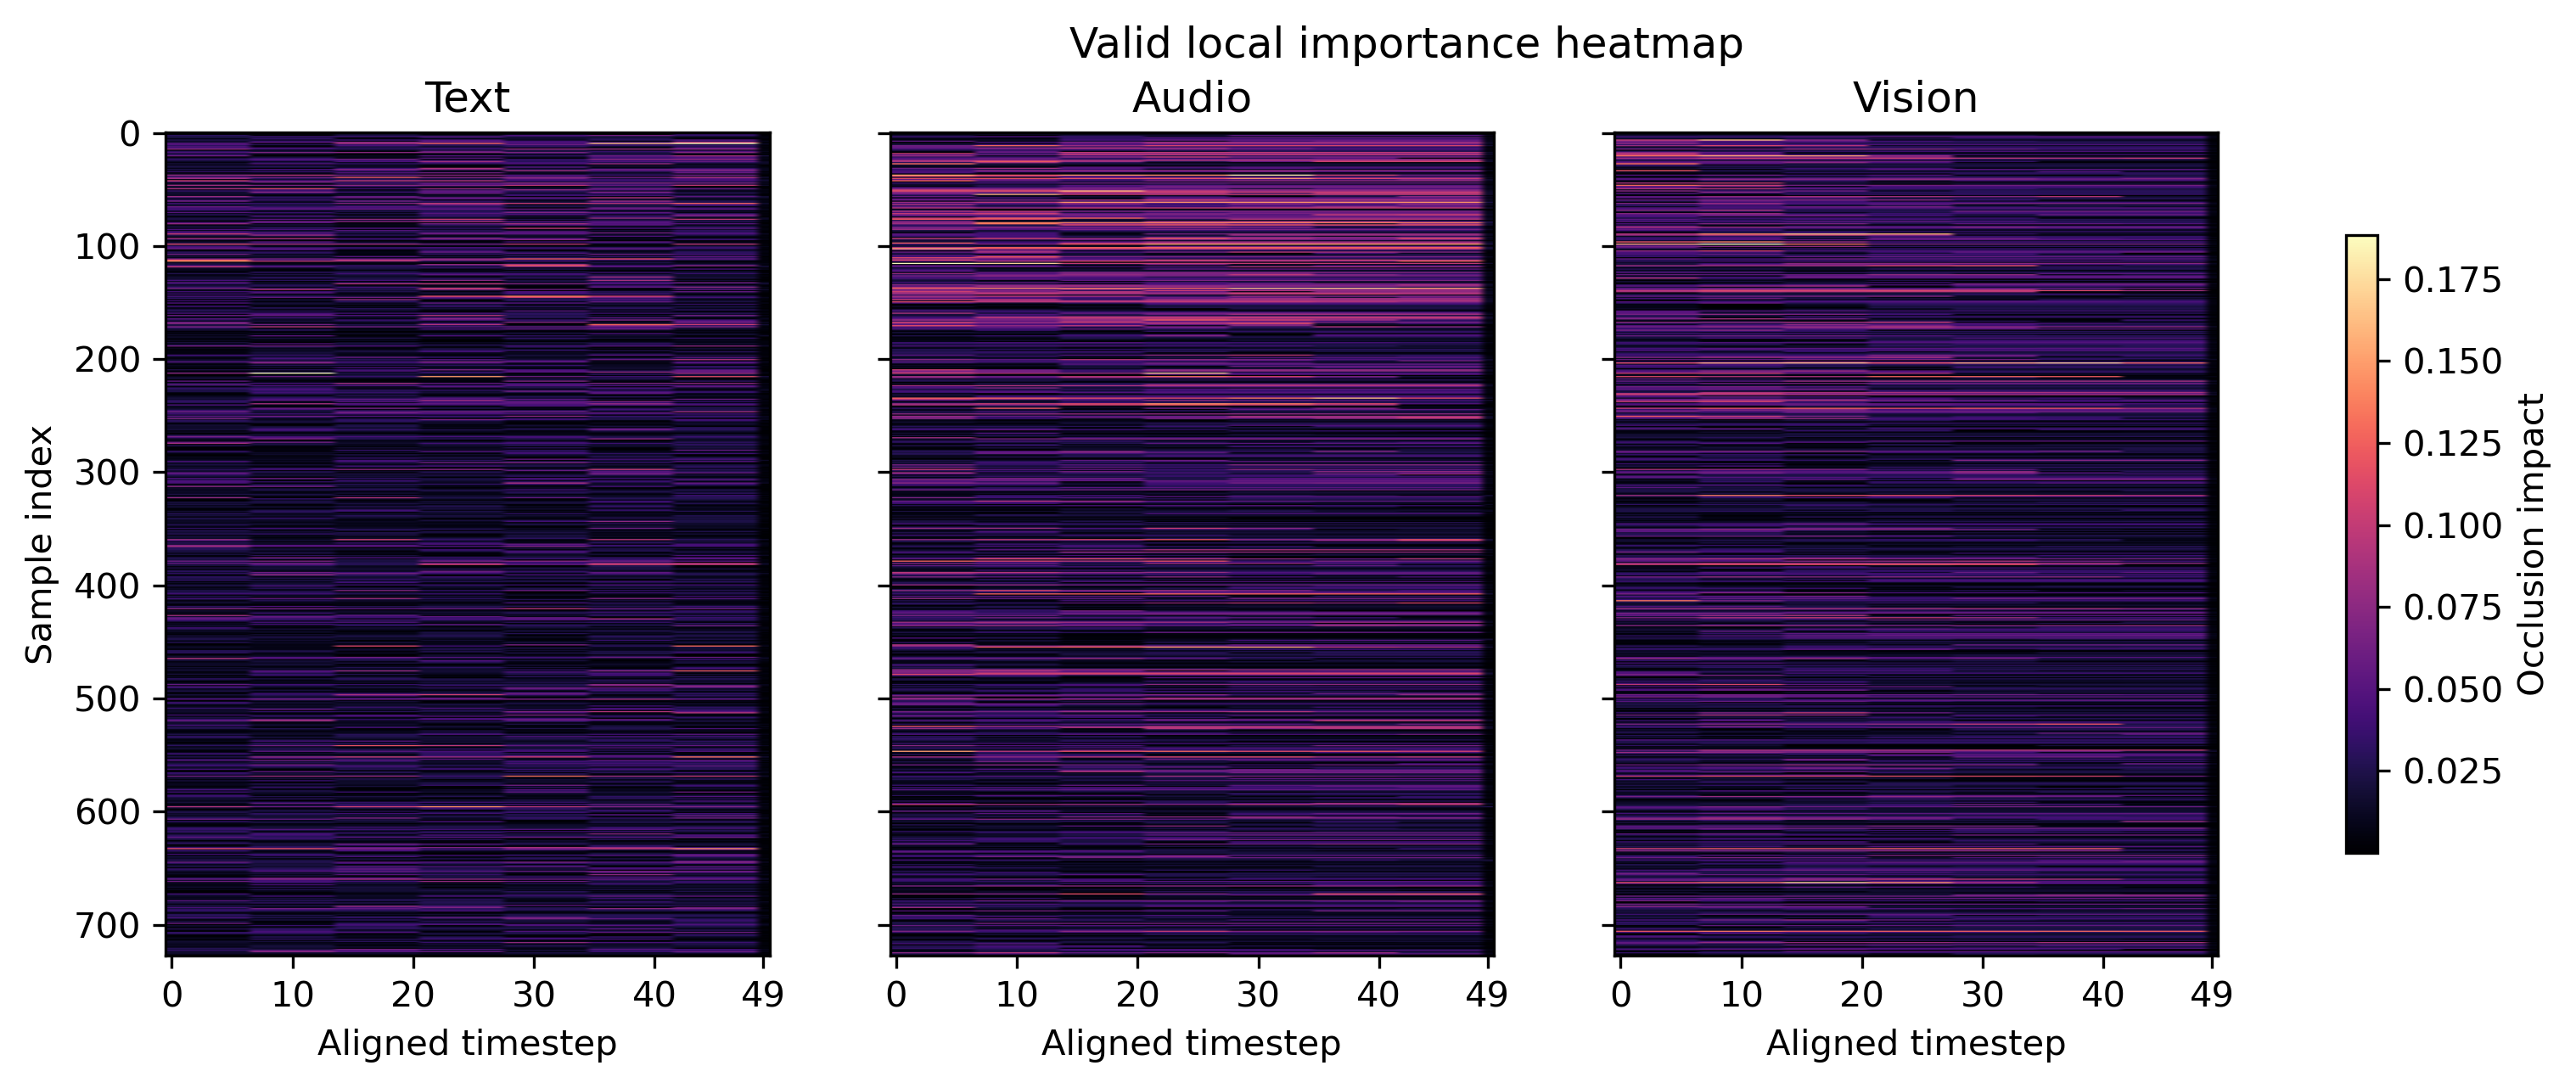
\includegraphics{assets/fig_local_importance_heatmap_valid.png}
\caption{valid 局部重要性}\label{fig:localvalid}
}
\end{figure}

\begin{figure}
\hypertarget{fig:localtest}{%
\centering
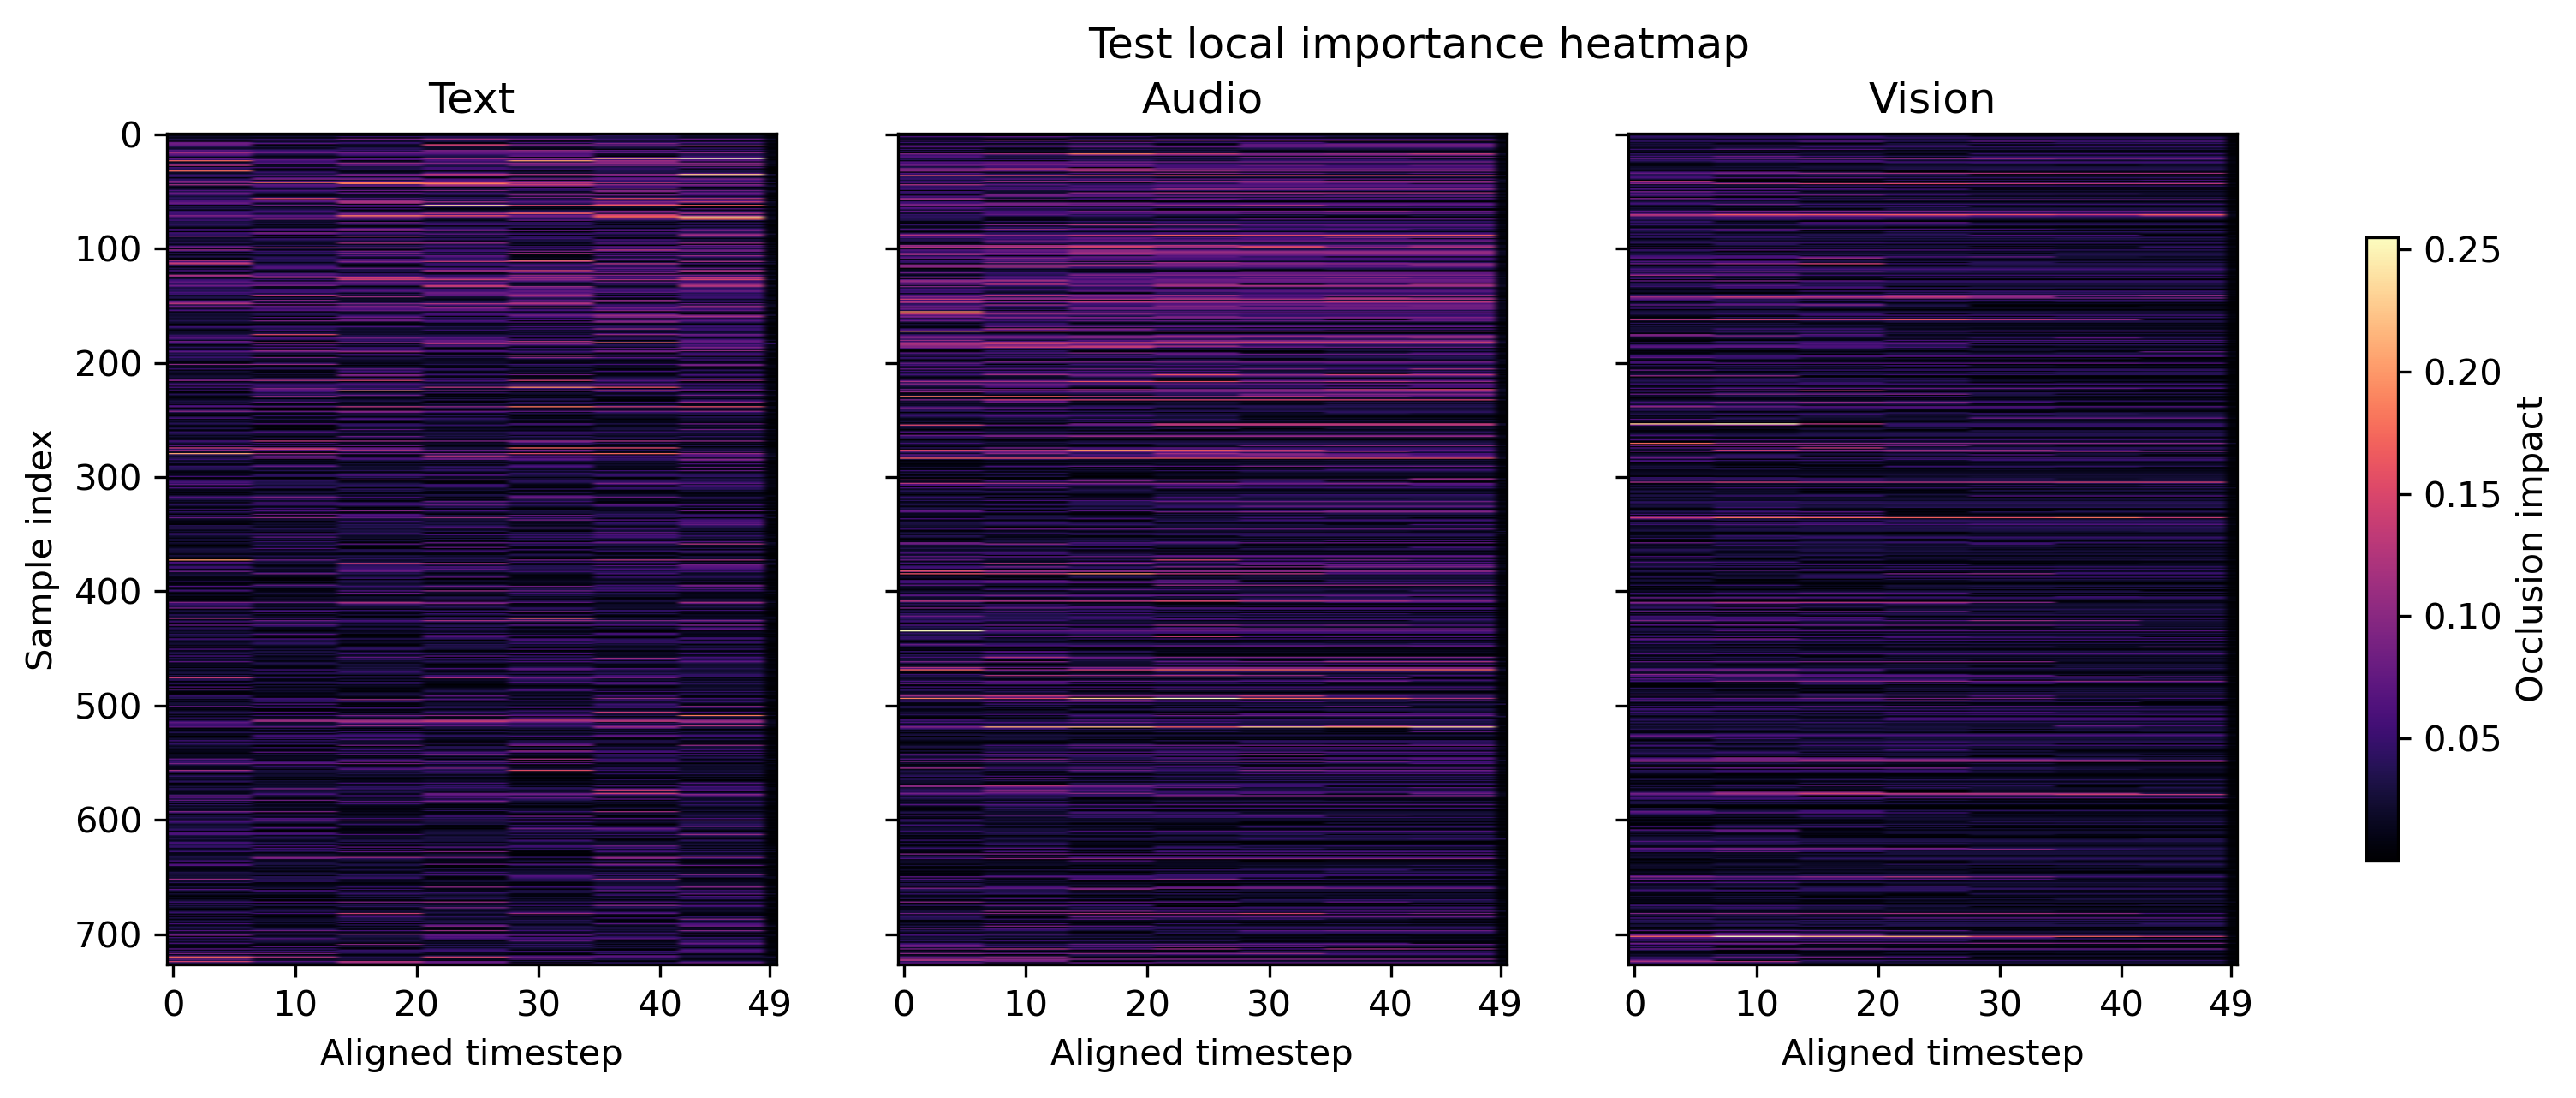
\includegraphics{assets/fig_local_importance_heatmap_test.png}
\caption{test 局部重要性}\label{fig:localtest}
}
\end{figure}

\begin{figure}
\hypertarget{fig:locala4}{%
\centering
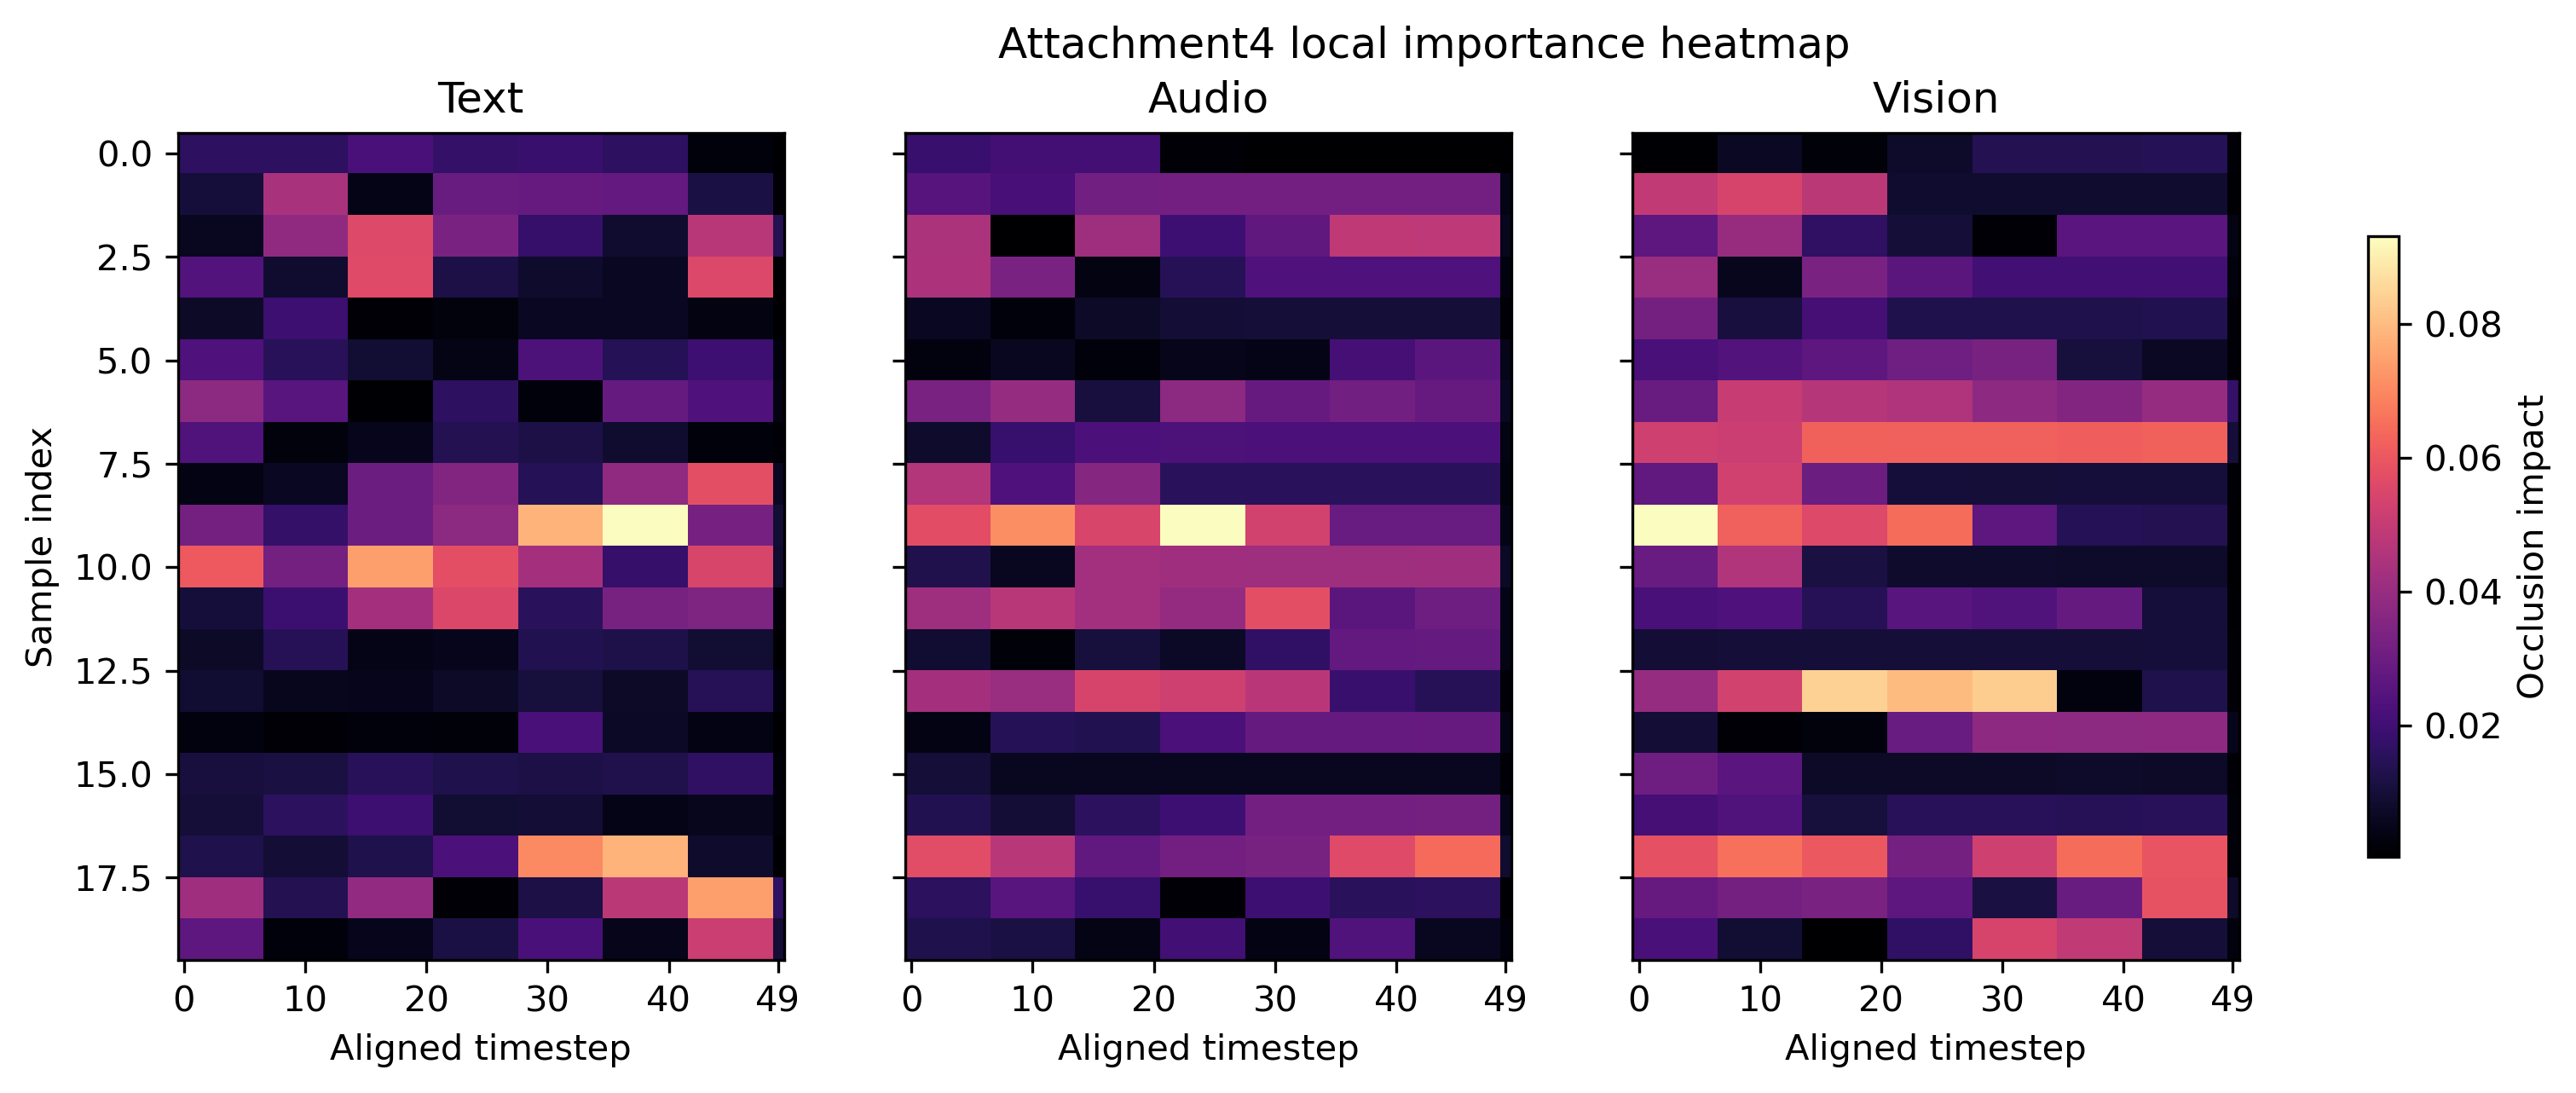
\includegraphics{assets/fig_local_importance_heatmap_attachment4.png}
\caption{附件四局部重要性}\label{fig:locala4}
}
\end{figure}

图 14--16
的横轴是对齐窗口位置，纵轴是样本，颜色表示反事实遮挡影响。它们提供的是可回溯的模型证据排序，不应被表述为逐词情感原因。

\hypertarget{ux4ee3ux8868ux6027ux6837ux672c}{%
\subsubsection{9.2 代表性样本}\label{ux4ee3ux8868ux6027ux6837ux672c}}

\textbf{表 5 代表性验证样本}

{\tiny
\begin{longtable}[]{@{}llllll@{}}
\toprule
类型 & sample\_id & 真实/预测类别 & 真实/预测强度 & 主要模态 &
文本/音频/视觉贡献 \\
\midrule
\endhead
文本主导 & \texttt{jICmfLeFymA\$\_\$16} & 2 / 2 & 1.667 / 1.029 & text &
0.976 / 0.005 / 0.018 \\
音频主导 & \texttt{PboaYD5hlG8\$\_\$8} & 0 / 2 & -1.333 / 0.338 & audio
& 0.167 / 0.735 / 0.098 \\
视觉主导 & \texttt{wosolsrH3sM\$\_\$6} & 2 / 0 & 0.333 / -0.763 & vision
& 0.092 / 0.159 / 0.749 \\
分类错误 & \texttt{0utROiKxejc\$\_\$1} & 1 / 2 & 0 / -0.016 & text &
0.582 / 0.206 / 0.212 \\
回归误差最大 & \texttt{252998\$\_\$7} & 2 / 0 & 1.333 / -1.996 & text &
0.603 / 0.061 / 0.337 \\
贡献均衡 & \texttt{TYJzg5IJN8o\$\_\$11} & 0 / 2 & -0.333 / 0.380 & audio
& 0.335 / 0.345 / 0.320 \\
\bottomrule
\end{longtable}
}

表 5 来自
\texttt{representative\_sample\_selection.csv}。其中音频主导和视觉主导样本均出现分类错误，说明主要模态是模型的依赖来源而不是正确性保证；该表因此同时承担解释案例和失败案例的作用。

\hypertarget{ux9644ux4ef6ux56dbux6700ux7ec8ux63a8ux7406}{%
\subsubsection{9.3
附件四最终推理}\label{ux9644ux4ef6ux56dbux6700ux7ec8ux63a8ux7406}}

附件四预测结果保存在 \texttt{predictions\_attachment4.csv}，20
条样本均生成类别、强度、门控、模态贡献、Top-3
证据影响和解释配置。代表性输出如下：样本 01 预测 Positive、强度
0.6411、主要模态 text；样本 02 预测 Negative、强度 -0.0867、主要模态
audio；样本 18 预测 Positive、强度 -1.0973、主要模态 vision；样本 16
预测 Negative、强度 -2.6106、主要模态
text。类别和连续强度是两个输出，不能仅根据类别推断强度符号。

\textbf{表 6 附件四代表性证据}

\begin{longtable}[]{@{}llrllr@{}}
\toprule
样本 & 预测类别 & 强度 & 主要模态 & Top-1 证据区间（秒） & 影响 \\
\midrule
\endhead
01 & Positive & 0.6411 & text & 2.520--3.780 & 0.0478 \\
02 & Negative & -0.0867 & audio & 0.471--0.943 & 0.0974 \\
09 & Negative & -1.9809 & text & 4.228--4.933 & 0.1281 \\
16 & Negative & -2.6106 & text & 2.604--3.038 & 0.0362 \\
18 & Positive & -1.0973 & vision & 13.090--15.708 & 0.1737 \\
\bottomrule
\end{longtable}

表 6 取自 \texttt{table\_evidence\_examples.csv}；完整 20
条记录和证据文本在 \texttt{evidence\_mapping\_attachment4.csv}
中。每个样本均有一张解释卡和三个以内的模态关键帧，\texttt{keyframes.json}
与 \texttt{evidence\_cards.json} 用文件名记录了元数据对应关系。

\begin{figure}
\hypertarget{fig:decode}{%
\centering
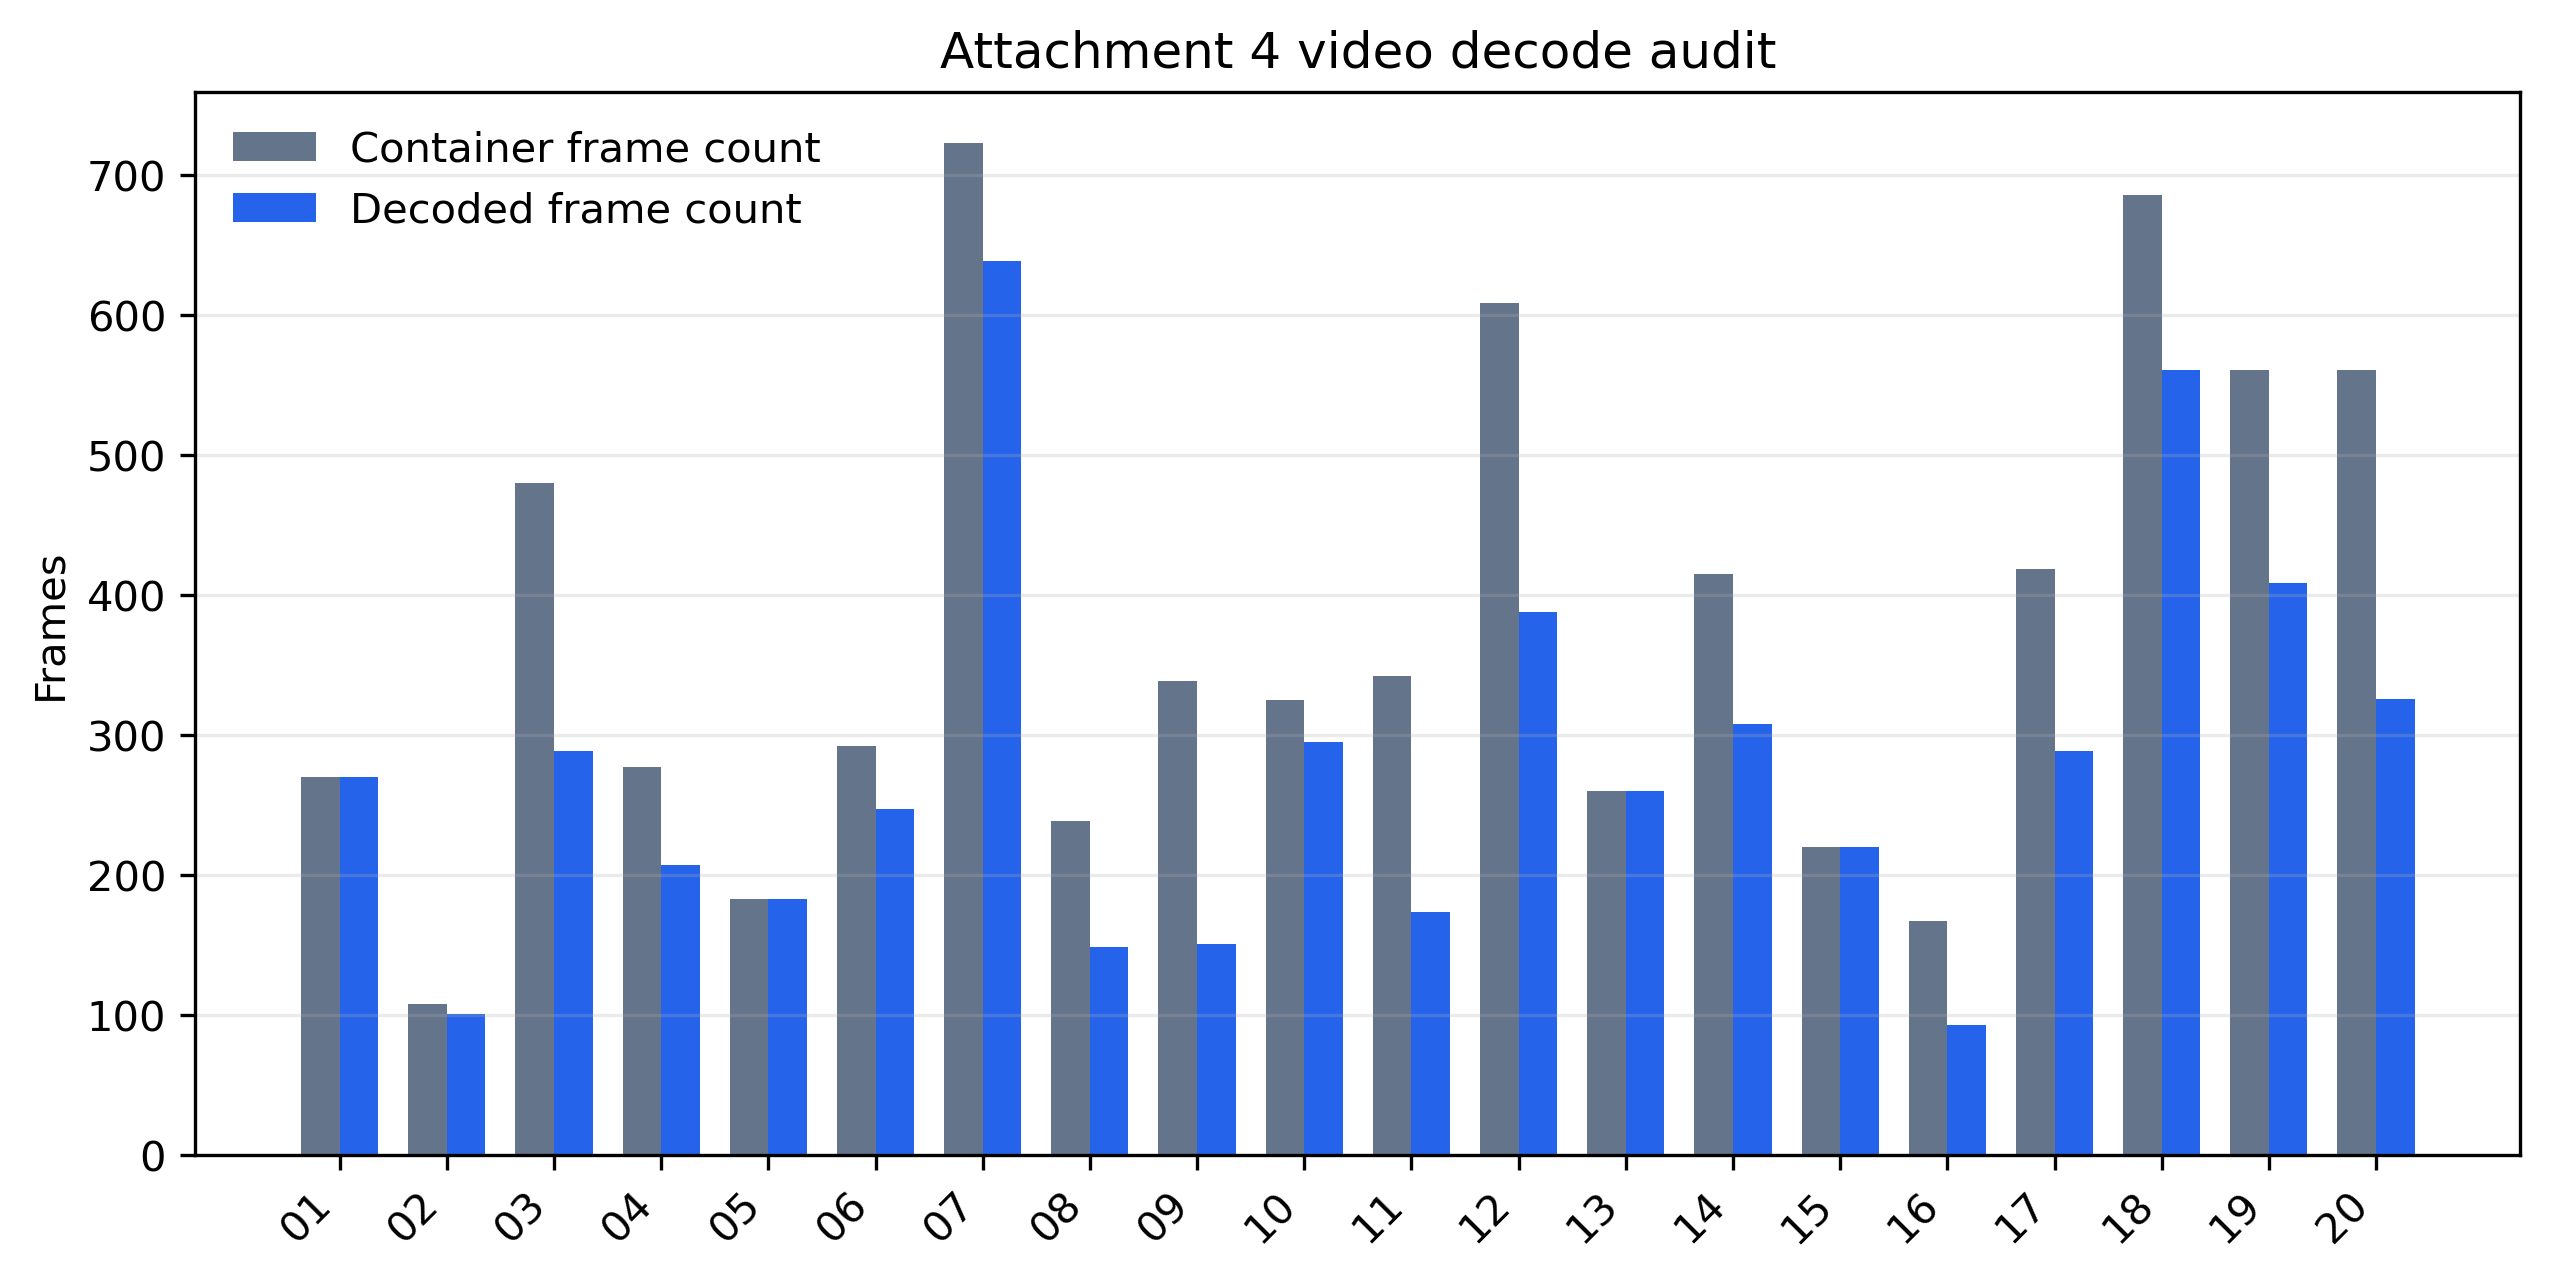
\includegraphics{assets/fig_video_decode_audit.png}
\caption{附件四视频解码审计}\label{fig:decode}
}
\end{figure}

图 17 是视频解码审计。20 个视频均能完成解码，但 16
个视频的容器声明帧数与实际解码帧数不一致；因此证据边界以实际解码帧数为准，并在审计文件中保留该异常。

\hypertarget{ux8bbaux6587ux652fux6491ux6750ux6599ux4e0eux53efux590dux73b0ux6027}{%
\subsection{10
论文支撑材料与可复现性}\label{ux8bbaux6587ux652fux6491ux6750ux6599ux4e0eux53efux590dux73b0ux6027}}

当前结果包中的图、表、数据和审计材料形成如下对应关系：

{\small
\begin{longtable}[]{@{}
  >{\raggedright\arraybackslash}p{(\columnwidth - 2\tabcolsep) * \real{0.50}}
  >{\raggedright\arraybackslash}p{(\columnwidth - 2\tabcolsep) * \real{0.50}}@{}}
\toprule
论文内容 & 实际支撑文件 \\
\midrule
\endhead
技术路线、模型结构、数据边界 &
\texttt{fig\_technical\_route.png}、\texttt{fig\_model\_architecture.png}、\texttt{fig\_data\_boundary.png} \\
训练过程 &
\texttt{training\_curve.csv}、\texttt{fig\_training\_curve.png} \\
分类与回归性能 &
\texttt{model\_metrics.csv}、\texttt{classification\_report\_valid.csv}、混淆矩阵和回归诊断图 \\
模态贡献与移除诊断 &
\texttt{modality\_contribution\_summary.csv}、\texttt{modality\_ablation\_metrics.csv}、\texttt{fig\_global\_contribution.png} \\
解释忠实性 &
\texttt{explanation\_parameter\_selection.json}、\texttt{fidelity\_metrics.json}、\texttt{fig\_fidelity\_valid.png} \\
局部证据 &
\texttt{local\_importance\_*.csv}、\texttt{evidence\_mapping\_*.csv}、局部重要性热力图 \\
附件四案例 &
\texttt{predictions\_attachment4.csv}、\texttt{table\_evidence\_examples.csv}、\texttt{keyframes/}、\texttt{evidence\_cards/} \\
数据质量与边界 &
\texttt{validation\_audit.json}、\texttt{video\_decode\_audit.csv}、\texttt{v8\_audit.json}、\texttt{final\_package\_audit.json} \\
\bottomrule
\end{longtable}
}

结果审计显示：输出均为有限值，train/valid/test
主键互不交叉，附件四完整生成 20
条预测，证据贡献可归一化，关键帧和解释卡与 JSON
元数据一一对应，附件四未参与训练或解释参数选择。模型权重、标准化参数、运行配置、训练日志和校验摘要共同构成复现材料。

\hypertarget{ux7ed3ux679cux8fb9ux754cux4e0eux5c40ux9650ux6027}{%
\subsection{11
结果边界与局限性}\label{ux7ed3ux679cux8fb9ux754cux4e0eux5c40ux9650ux6027}}

第一，当前没有不同网络结构的重新训练基线，表 4
不能替代完整消融实验。第二，主要结果来自单一随机种子，未报告多种子均值、标准差和置信区间。第三，文本定位是对齐相对窗口，不是逐词时间戳。第四，附件四视频存在容器帧数和实际解码帧数不一致，关键帧解释必须结合视频审计。第五，门控值、注意力权重和
\texttt{impact\_score}
都是模型内部状态或后验敏感性，不是人工标注的真实情感原因。第六，附件四无标签，任何性能评价只能停留在附件二
valid/test。

上述限制不否定当前输出对论文撰写的作用，但要求论文对``模型表现''``模型依赖''``证据映射''和``真实情感原因''进行严格区分。所有指标、图表和案例均应以结果包中的文件为准，不补写未运行的实验结论。

\end{document}
